%
% Template Laporan Skripsi/Thesis 
%
% @author  Andreas Febrian, Lia Sadita 
% @version 1.03
%
% Dokumen ini dibuat berdasarkan standar IEEE dalam membuat class untuk 
% LaTeX dan konfigurasi LaTeX yang digunakan Fahrurrozi Rahman ketika 
% membuat laporan skripsi. Konfigurasi yang lama telah disesuaikan dengan 
% aturan penulisan thesis yang dikeluarkan UI pada tahun 2008.
%

%
% Tipe dokumen adalah report dengan satu kolom. 
%
\documentclass[12pt, a4paper, onecolumn, oneside, final]{report}

% Load konfigurasi LaTeX untuk tipe laporan thesis
%\usepackage{uithesis}
\usepackage{uithesismod}

% Load konfigurasi khusus untuk laporan yang sedang dibuat
%-----------------------------------------------------------------------------%
% Informasi Mengenai Dokumen
%-----------------------------------------------------------------------------%
% 
% Judul laporan. 
\var{\judul}{Efek Fluktuasi Okupasi pada Model Hubbard 3D dalam Kerangka Dynamical Mean-Field Theory}
% 
% Tulis kembali judul laporan, kali ini akan diubah menjadi huruf kapital
\Var{\Judul}{EFEK FLUKTUASI OKUPASI PADA MODEL HUBBARD 3D DALAM KERANGKA DYNAMICAL MEAN-FIELD THEORY}
% 
% Tulis kembali judul laporan namun dengan bahasa Ingris
\var{\judulInggris}{Occupation Fluctuation Effect on 3D Hubbard Model within Dynamical Mean-Field Theory Framework}

% 
% Tipe laporan, dapat berisi Skripsi, Tugas Akhir, Thesis, atau Disertasi
\var{\type}{Skripsi}
% 
% Tulis kembali tipe laporan, kali ini akan diubah menjadi huruf kapital
\Var{\Type}{SKRIPSI}
% 
% Tulis nama penulis 
\var{\penulis}{Muhammad Gaffar As Shiddieqy Al Anshori}
% 
% Tulis kembali nama penulis, kali ini akan diubah menjadi huruf kapital
\Var{\Penulis}{MUHAMMAD GAFFAR AS SHIDDIEQY AL ANSHORI}
% 
% Tulis NPM penulis
\var{\npm}{1506724322}
% 
% Tuliskan Fakultas dimana penulis berada
\Var{\Fakultas}{Matematika dan Ilmu Pengetahuan Alam}
\var{\fakultas}{Matematika dan Ilmu Pengetahuan Alam}
% 
% Tuliskan Program Studi yang diambil penulis
\Var{\Program}{Fisika}
\var{\program}{Fisika}
% 
% Tuliskan tahun publikasi laporan
\Var{\bulanTahun}{Juli 2019}
% 
% Tuliskan gelar yang akan diperoleh dengan menyerahkan laporan ini
\var{\gelar}{Sarjana Sains}
% 
% Tuliskan tanggal pengesahan laporan, waktu dimana laporan diserahkan ke 
% penguji/sekretariat
\var{\tanggalPengesahan}{20 Juni 2019} 
% 
% Tuliskan tanggal keputusan sidang dikeluarkan dan penulis dinyatakan 
% lulus/tidak lulus
\var{\tanggalLulus}{28 Juni 2019}
% 
% Tuliskan pembimbing 
\var{\pembimbing}{Muhammad Aziz Majidi, Ph.D}
% 
% Alias untuk memudahkan alur penulisan paa saat menulis laporan
\var{\saya}{Muhammad Gaffar As. A.}

%-----------------------------------------------------------------------------%
% Judul Setiap Bab
%-----------------------------------------------------------------------------%
% 
% Berikut ada judul-judul setiap bab. 
% Silahkan diubah sesuai dengan kebutuhan. 
% 
\Var{\kataPengantar}{Kata Pengantar}
\Var{\babSatu}{Pendahuluan}
\Var{\babDua}{Tinjauan Pustaka}
\Var{\babTiga}{Metode}
\Var{\babEmpat}{Hasil dan Diskusi}
\Var{\babLima}{Kesimpulan dan Saran}
% Daftar pemenggalan suku kata dan istilah dalam LaTeX
%
% Hyphenation untuk Indonesia 
%
% @author  Andreas Febrian
% @version 1.00
% 
% Tambahkan cara pemenggalan kata-kata yang salah dipenggal secara otomatis 
% oleh LaTeX. Jika kata tersebut dapat dipenggal dengan benar, maka tidak 
% perlu ditambahkan dalam berkas ini. Tanda pemenggalan kata menggunakan 
% tanda '-'; contoh:
% menarik
%   --> pemenggalan: me-na-rik
%

\hyphenation{
    % alphabhet A
    a-na-li-sa a-tur 
    a-pli-ka-si 
    % alphabhet B
    ba-ngun-an 
    be-be-ra-pa 
    ber-ge-rak
    ber-ke-lan-jut-an 
    ber-pe-nga-ruh 
    % alphabhet C
    ca-ri
    % alphabhet D
    di-sim-pan di-pim-pin de-ngan da-e-rah di-ba-ngun da-pat di-nya-ta-kan 
    di-sim-bol-kan di-pi-lih di-li-hat de-fi-ni-si
    % alphabhet E
    e-ner-gi eks-klu-sif
    % alphabhet F
    fa-si-li-tas
    % alphabhet G
    ga-bung-an ge-rak
    % alphabhet H
    ha-lang-an
    % alphabhet I
    % alphabhet J
    % alphabhet K
    ke-hi-lang-an
    ku-ning 
    kua-li-tas ka-me-ra ke-mung-kin-an ke-se-pa-ham-an
    % alphabhet L
    ling-kung-an
    % alphabhet M
    me-neng-ah
    meng-a-tas-i me-mung-kin-kan me-nge-na-i me-ngi-rim-kan 
    meng-u-bah meng-a-dap-ta-si me-nya-ta-kan mo-di-fi-ka-si
    meng-a-tur
    % alphabhet N
    nya-ta non-eks-klu-sif
    % alphabhet O
    % alphabhet P
	pe-nye-rap-an 
	pe-ngon-trol
    pe-mo-del-an
    pe-ran  pe-ran-an-nya
    pem-ba-ngun-an pre-si-den pe-me-rin-tah prio-ri-tas peng-am-bil-an 
    peng-ga-bung-an pe-nga-was-an pe-ngem-bang-an 
    pe-nga-ruh pa-ra-lel-is-me per-hi-tung-an per-ma-sa-lah-an 
    pen-ca-ri-an peng-struk-tur-an
    % alphabhet Q
    % alphabhet R
    ran-cang-an
    % alphabhet S
    si-mu-la-si sa-ngat
    % alphabhet T
    te-ngah
    ter-da-pat
    % alphabhet U
    % alphabhet V
    % alphabhet W
    % alphabhet X
    % alphabhet Y
    % alphabhet Z
    % special
}
% Daftar istilah yang mungkin perlu ditandai 
%
% @author  Andreas Febrian
% @version 1.00
% 
% Mendaftar seluruh istilah yang mungkin akan perlu dijadikan 
% italic atau bold pada setiap kemunculannya dalam dokumen. 
% 

\var{\license}{\f{Creative Common License 1.0 Generic}}
\var{\bslash}{$\setminus$}

% Awal bagian penulisan laporan
\begin{document}
%
% Sampul Laporan
%
% Sampul Laporan

%
% @author  unknown
% @version 1.01
% @edit by Andreas Febrian
%

\begin{titlepage}
    \begin{center}    
        \begin{figure}
            \begin{center}
                \includegraphics[width=2.5cm]{pics/makara.png}
            \end{center}
        \end{figure}    
        \vspace*{0cm}
        \bo{
        	UNIVERSITAS INDONESIA\\
        }
        
        \vspace*{1.0cm}
        % judul thesis harus dalam 14pt Times New Roman
        \bo{\Judul} \\[1.0cm]

        \vspace*{2.5 cm}    
        % harus dalam 14pt Times New Roman
        \bo{\Type}

        \vspace*{3 cm}       
        % penulis dan npm
        \bo{\Penulis} \\
        \bo{\npm} \\

        \vspace*{5.0cm}

        % informasi mengenai fakultas dan program studi
        \bo{
        	FAKULTAS \Fakultas\\
        	PROGRAM STUDI \Program \\
        	DEPOK \\
        	\bulanTahun
        }
    \end{center}
\end{titlepage}


%
% Gunakan penomeran romawi
\pagenumbering{roman}

%
% load halaman judul dalam
\addChapter{HALAMAN JUDUL}
%
% Halaman Judul Laporan 
%
% @author  unknown
% @version 1.01
% @edit by Andreas Febrian
%

\begin{titlepage}
    \begin{center}\begin{figure}
            \begin{center}
                \includegraphics[width=2.5cm]{pics/makara.png}
            \end{center}
        \end{figure}    
        \vspace*{0cm}
        \bo{
        	UNIVERSITAS INDONESIA\\
        }
        
        \vspace*{1.0cm}
        % judul thesis harus dalam 14pt Times New Roman
        \bo{\Judul} \\[1.0cm]

        \vspace*{2.5 cm}    
        % harus dalam 14pt Times New Roman
        \bo{\Type} \\
        % keterangan prasyarat
        \bo{Diajukan sebagai salah satu syarat untuk memperoleh gelar \\
        \gelar}\\

        \vspace*{3 cm}       
        % penulis dan npm
        \bo{\Penulis} \\
        \bo{\npm} \\

        \vspace*{5.0cm}

        % informasi mengenai fakultas dan program studi
        \bo{
        	FAKULTAS \Fakultas\\
        	PROGRAM STUDI \Program \\
        	DEPOK \\
        	\bulanTahun
        }
    \end{center}
\end{titlepage}

%
% setelah bagian ini, halaman dihitung sebagai halaman ke 2
\setcounter{page}{2}

%
% load halaman pengesahan
\addChapter{LEMBAR PERSETUJUAN}
%%
% Halaman Pengesahan
%
% @author  Andreas Febrian
% @version 1.01
%

\chapter*{HALAMAN PERSETUJUAN}

\vspace*{0.2cm}
\noindent 

\noindent
\begin{tabular}{l l p{11cm}}
	\bo{Judul}&: & \judul \\ 
	\bo{Nama}&: & \penulis \\
	\bo{NPM}&: & \npm \\
\end{tabular} \\

\vspace*{1.2cm}

\noindent Laporan \type~ini telah diperiksa dan disetujui.\\[0.3cm]
\begin{center}
\tanggalPengesahan \\[2cm]


\underline{\pembimbing}\\[0.1cm]
Pembimbing \type
\end{center}

\newpage
%
% load halaman orisinalitas 
\addChapter{LEMBAR PERNYATAAN ORISINALITAS}
%
% Halaman Orisinalitas
%
% @author  Andreas Febrian
% @version 1.01
%

\chapter*{\uppercase{halaman pernyataan orisinalitas}}
\vspace*{2cm}

\begin{center}
	\bo{\type~ini adalah hasil karya saya sendiri, \\ 
	dan semua sumber baik yang dikutip maupun dirujuk \\
	telah saya nyatakan dengan benar.} \\
	\vspace*{2.6cm}
	
	\begin{tabular}{l c l}
	\bo{Nama} & : & \bo{\penulis} \\
	\bo{NPM} & : & \bo{\npm} \\ 
	\bo{Tanda Tangan} & : & \\
	& & \\
	& & \\
	\bo{Tanggal} & : & \bo{\tanggalPengesahan} \\	
	\end{tabular}
\end{center}

\newpage
%
%
\addChapter{LEMBAR PENGESAHAN}
%
% Halaman Pengesahan Sidang
%
% @author  Andreas Febrian, Andre Tampubolon 
% @version 1.02
%

\chapter*{HALAMAN PENGESAHAN}

\vspace*{0.4cm}
\noindent 

\noindent
\begin{tabular}{ll p{9cm}}
	\type~ini diajukan oleh&: & \\
	Nama&: & \penulis \\
	NPM&: & \npm \\
	Program Studi&: & \program \\
	Judul \type&: & \judul \\
\end{tabular} \\

\vspace*{1.0cm}

\noindent \bo{Telah berhasil dipertahankan di hadapan Dewan Penguji 
dan diterima sebagai bagian persyaratan yang diperlukan untuk 
memperoleh gelar \gelar~pada Program Studi \program, Fakultas 
\fakultas, Universitas Indonesia.}\\[0.2cm]

\begin{center}
	\bo{DEWAN PENGUJI}
\end{center}

\vspace*{0.3cm}

\begin{tabular}{l l l l }
	& & & \\
	Pembimbing&: & \pembimbing & (\hspace*{3.0cm}) \\
	& & & \\
	Penguji&: & Efta Yudiarsah, Ph.D & (\hspace*{3.0cm}) \\
	& & & \\
	Penguji&: & Dr. Adam Badra Cahaya & (\hspace*{3.0cm}) \\
\end{tabular}\\

\vspace*{2.0cm}

\begin{tabular}{ll l}
	Ditetapkan di&: & Depok\\
	Tanggal&: & \tanggalLulus \\
\end{tabular}


\newpage
%
%
\addChapter{\kataPengantar}
%-----------------------------------------------------------------------------%
\chapter*{\kataPengantar}
%-----------------------------------------------------------------------------%
Pertama-tama, saya ucapkan rasa syukur kepada Allah SWT, dikarenakan kasih sayang dan rahmat-Nya, saya dapat menyelesaikan skripsi tepat waktu. Shalawat beserta salam disampaikan juga kepada Rasulullah Muhammad SAW, junjungan seluruh Alam, beserta keluarga, dan sahabatnya, dikarenakan proses pengajaran ilmu dari generasi merekalah saya bisa mengenal Islam sebagai \textit{rahmatan lil alamin}. 

Proses skripsi yang ditujukan untuk mendapatkan gelar sarjana sains ini tidak lepas berkat kontribusi dan dukungan banyak pihak. Secara khusus, saya ucapkan terima kasih kepada:
\begin{enumerate}
	\item Muhammad Aziz Majidi, Ph.D yang telah menjadi pembimbing saya dalam menjalani
	studi dan riset di peminatan fisika zat mampat. Berkat bimbingannya, saya mendapatkan
	banyak ilmu dan motivasi dalam menjalani skripsi saya.
	\item Kepada kedua orangtua saya, Eddy Asnawi dan Zetriuslita, dan kedua adik saya, Muhammad Luthfi 
	Taufiqqurahman dan Muhammad Aziz Habiburrahim yang selalu mendoakan saya.
	\item Choirun Nisaa Rangkuti, sebagai mentor riset saya yang telah membantu membimbing saya
	dalam penulisan komputasi numerik pada awal-awal riset skripsi ini dimulai. 
	\item Teman-teman anggota lab \textit{Theoretical Condensed Matter Physics} (TCMP) yang telah
	menemani dalam suka dan duka selama rentang pengerjaan riset skripsi. Terkhususnya angkatan 2015, 
	1) Wilwin sebagai teman yang sangat memotivasi saya mengejar hal-hal akademik dan diskusi mengenai fisika,
	2) Dedi Prakasa sebagai teman yang unik dan lucu, 3) Andes Rogata Parmonangan Tambunan sebagai teman seperjuangan dan senasib
	dalam studi fisika, dan 4) Nur Atikah Tadjuddin sebagai teman pengerjaan satu topik riset.
	\item Teman-teman fisika non-TCMP lainnya, 1) Benedictus Bayu Respati sebagai teman dan sahabat yang luar biasa
	dalam berdiskusi mengenai perkuliahan dan kegiatan non-akademis.	2) Muhammad Mahdi Ramadhan sebagai teman pertama dan sahabat yang kaya pikiran yang selalu penuh dengan kejutan disaat berdiskusi, 3) Jason Kristiano, Agya Sewara Alam, sebagai teman yang menemani saya dalam 	diskusi mengenai fisika, 4) Faidzal Adilla, Ahmad Fauzan Kamaluddin, Faiz Rambey, Naufal Praditya, Reyan Qowi, Eufrat Tsaqib, Rasyid Sulaeman, dan Nabilah Hana Luthfiyah sebagai teman-teman yang pernah menemani saya dalam berbagai kegiatan di kampus,	dan 5) Abyan Jadiddan, Feby Nirwana, dan Indrianita Lionardi sebagai teman yang menjadi inspirasi saya untuk terus berbuat baik, dan bersikap rendah hati. Terakhir tentu, semua angkatan Fisika 2015 yang menjadi angkatan yang dinamis dalam menemani saya dalam 4 tahun studi fisika.
\end{enumerate}
Saya juga berterima kasih kepada semua orang yang telah banyak mendewasakan diri saya dalam menjalani perkuliahan, baik
dalam akademis maupun non-akademis. Saya berharap hasil skripsi saya ini akan berguna bagi siapa saja yang membacanya.

\vspace*{0.1cm}
\begin{flushright}
Depok, 28 Juni 2019\\[0.1cm]
\vspace*{1cm}
\penulis

\end{flushright}	
%
%
\addChapter{LEMBAR PERSETUJUAN PUBLIKASI ILMIAH}
% 
% @author  Andre Tampubolon, Andreas Febrian
% @version 1.01
% 

\chapter*{\uppercase{Halaman Pernyataan Persetujuan Publikasi Tugas Akhir untuk Kepentingan Akademis}}

\vspace*{0.2cm}
\noindent 
Sebagai sivitas akademik Universitas Indonesia, saya yang bertanda 
tangan di bawah ini:
\vspace*{0.4cm}


\begin{tabular}{p{4.2cm} l p{6cm}}
	\bo{Nama} & : & \penulis \\ 	
	\bo{NPM} & : & \npm \\
	\bo{Program Studi} & : & \program\\	
	\bo{Fakultas} & : & \fakultas\\
	\bo{Jenis Karya} & : & \type \\
\end{tabular}

\vspace*{0.6cm}
\noindent demi pengembangan ilmu pengetahuan, menyetujui untuk memberikan 
kepada Universitas Indonesia \bo{Hak Bebas Royalti Noneksklusif 
(Non-exclusive Royalty Free Right)} atas karya ilmiah saya yang berjudul:
\begin{center}
	\judul
\end{center}
beserta perangkat yang ada (jika diperlukan). Dengan Hak Bebas Royalti 
Noneksklusif ini Universitas Indonesia berhak menyimpan, 
mengalihmedia/formatkan, mengelola dalam bentuk pangkalan data 
(database), merawat, dan memublikasikan tugas akhir saya selama 
tetap mencantumkan nama saya sebagai penulis/pencipta dan sebagai 
pemilik Hak Cipta. \\

\noindent Demikian pernyatan ini saya buat dengan sebenarnya.

\begin{center}
	\vspace*{0.8cm}
	\begin{tabular}{lll}
		Dibuat di&: & Depok \\
		Pada tanggal&: & \tanggalPengesahan \\
	\end{tabular}\\

	\vspace*{0.2cm}
	Yang menyatakan \\
	\vspace*{1.1cm}
	(\penulis)
\end{center}

\newpage


%
%
\addChapter{ABSTRAK}
%
% Halaman Abstrak
%
% @author  Andreas Febrian
% @version 1.00
%

\chapter*{Abstrak}

\vspace*{0.2cm}

\noindent \begin{tabular}{l l p{10cm}}
	Nama&: & \penulis \\
	Program Studi&: & \program \\
	Judul&: & \judul \\
\end{tabular} \\ 

\vspace*{0.5cm}

\noindent \todo{Tuliskan abstrak laporan disini.} \\

\vspace*{0.2cm}

\noindent Kata Kunci: \\ 
\noindent \todo{Tuliskan kata kunci yang berhubungan dengan laporan 
	disini} \\

\newpage
%
% Halaman Abstract
%
% @author  Andreas Febrian
% @version 1.00
%

\chapter*{ABSTRACT}

\vspace*{0.2cm}

\noindent \begin{tabular}{l l p{11.0cm}}
	Name&: & \penulis \\
	Program&: & \program \\
	Title&: & \judulInggris \\
\end{tabular} \\ 

\vspace*{0.5cm}

\noindent \todo{Write your abstract here.}\\

\vspace*{0.2cm}

\noindent Keywords: \\ 
\noindent \todo{Write up keywords about your report here.}

\newpage
%
% Daftar isi, gambar, dan tabel
%
\tableofcontents
\clearpage
\listoffigures
\clearpage	
%
% Gunakan penomeran Arab (1, 2, 3, ...) setelah bagian ini.
%
\pagenumbering{arabic}

%
%
%
%-----------------------------------------------------------------------------%
\chapter{\babSatu}
%-----------------------------------------------------------------------------%

%-----------------------------------------------------------------------------%
\section{Latar Belakang}
%-----------------------------------------------------------------------------%
Model Drude \cite{drude} salah satu menjadi model pertama yang berhasil mendeskripsikan sifat-sifat fisis dari sebagian besar logam. Misalnya saja, model Drude dapat menjelaskan resistivitas residu pada temperatur rendah, suseptibilitas magnet yang tidak bergantung dengan temperatur, dan kapasitas panas yang bergantung  secara linear terhadap temperatur. Model Drude dijelaskan dengan mempertimbangkan elektron sebagai gas elektron yang tidak berinteraksi. Selanjutnya, model elektron hampir bebas (\textit{nearly free electron}) atau teori struktur pita energi\cite{ashcroft-mermin} memperbaiki model Drude, dimana mempertimbangkan potensial periodik dari kisi atomik. Hal ini tidak hanya dapat menjelaskan logam dengan baik, tetapi juga menjadi pendekatan yang kuat untuk menjelaskan material non-logam, yakni isolator dan semikonduktor. Perhitungan struktur pita energi telah terus diperluas pada situasi-situasi yang lebih realitis untuk elektron banyak-benda seperti memperhitungkan \textit{exchange mechanism} dan interaksi coulomb yang didekati secara medan rata-rata. Pendekatan medan rata-rata juga diketahui sebagai teori Hartree-Fock dimana fungsi gelombang benda-banyak ditulis dalam determinan slater. Namun, menghitung dengan determinan slater bisa menjadi sangat mahal dimana membutuhkan jangka waktu yang lama dikarenakan jumlah elektron yang diperhitungkan sangat banyak ($\sim 10^{22}$) pada situasi material asli. Metode alternatif kemudian dikembangkan oleh W.Kohn dan L.J.Sham\cite{kohn-sham}, yang dimana karena pendekatannya dapat ditulis energi dasar dari elektron banyak-benda sebagai fungsional densitas elektron. Pendekatan ini diketahui sebagai \textit{density functional theory} (DFT), yang dimana telah sukses memprediksi energi dasar berbagai material dalam beberapa dekade terakhir.

Walaupun DFT terbilang sangat sukses dalam menjelaskan sifat fisis dari berbagai material, masih terdapat kelompok material yang belum dapat terjelaskan dengan pendekatan tersebut, dan membutuhkan teori baru. Di tahun 1937, de Boer dan Verwey\cite{boer} memperlihat dalam eksperimennya bahwa adanya sifat isolator pada logam transisi oksida seperti NiO dan CoO walaupun orbital-$d$ yang belum terisi penuh di material tersebut diprediksi akan memiliki sifat logam dalam sudut pandang teori pita energi. Nevil Mott\cite{mott} berpendapat bahwa terdapat interaksi tolak-menolak Coulomb antar elektron yang menghalangi terjadinya sifat logam, sehingga material tersebut sebagai mott isolator. Mott isolator dapat dilihat pada logam \textit{Fermi liquid} saat adanya perubahan besar interaksi sehingga terjadi transisi logam-isolator (\textit{metal-insulator}) yang juga diketahui sebagai Transisi Mott. Logam yang memiliki Transisi Mott menunjukkan adanya resistivitas dan koefisien kapasitas panas yang tinggi. Tipe logam tersebut dikategorikan sebagai logam buruk (\textit{bad metal}) walaupun mereka memiliki sifat \textit{Fermi liquid}. Kategori material yang memiliki kontribusi interaksi Coulomb antar elektron yang tidak dapat diabaikan disebut sebagai material terkolerasi kuat.

Model Hubbard menjadi model paling sederhana yang dapat menangkap sifat fisis yang esensial pada material terkolerasi kuat dimulai dari transisi Mott-Hubbard logam-isolator\cite{mott-hubbard}, antiferomagnetik\cite{antiferomagnetik1}, dan superkonduktivitas $d$-\textit{wave}\cite{d-wave}. Meskipun minimnya solusi eksak dari model Hubbard, namun banyak terdapat pendeketan teoritis yang dilakukan secara aproksimasi. Salah satu metode yang paling ampuh dalam mengerjakan model Hubbard adalah \textit{Dynamical Mean-Field Theory}(DMFT)\cite{DMFT}. DMFT memiliki kesamaan dengan pendekatan medan rata-rata, keduanya memetakan masalah kisi banyak-benda ke site tunggal yang bersifat lokal. Metode ini menjadi eksak pada batas dimensi yang tak berhingga. 

DMFT pada dasarnya adalah memetakan kisi banyak-benda kuantum, seperti model Hubbard, ke model impuritas, dengan kondisi self-consistency. Hal ini menjadi sangat praktis dikarenakan pada batas dimensi tak berhingga \textit{self-energy} menjadi tidak bergantung dengan ruang momentum, dan hanya bergantung pada energi elektron, sehingga kuantitasnya bersifat lokal. Berbeda dengan DFT yang menggunakan densitas elektron sebagai salah satu kuantitas utamanya, DMFT dihitung pada formalisme fungsi Green. Model impuritas ini secara umum dapat diselesaikan banyak metode, diantaranya quantum Monte Carlo, Diagonalisasi Eksak, dan teori iterasi pertubasi. Namun, metode quantum Monte Carlo menggunakan metode komputasi yang sangat berat dikarenakan teknik samplingnya yang harus pada jumlah yang besar, sama halnya dengan Diagonalisasi Eksak yang membutuhkan sumber daya komputasi yang besar dikarenakan perhitungan total basis yang sangat besar pada situasi material asli sehingga ini biasanya dikerjakan pada sistem dengan ukuran terbatas, sedangkan teori iterasi pertubasi fluktuasi kuantum didekati secara pertubatif yang dimana ini menggunakan sumberdaya komputasi yang ringan namun tidak dapat menjelaskan pada daerah dengan interaksi coulomb yang kuat dimana pendekatan pertubasi tidak berlaku. Hingga saat ini masih dilakukan pengembangan perhitungan model impuritas yang akurat namun membutuhkan sumberdaya komputasi yang tidak besar.


%-----------------------------------------------------------------------------%
\section{Batas Permasalahan}
%-----------------------------------------------------------------------------%
Dibutuhkan pengembangan metode penyelesaian impuritas pada DMFT yang cukup akurat dan efektif namun menggunakan sumberdaya komputasi yang ringan. Metode ini dikembangkan atas dasar pengembangan lebih jauh dari medan rata-rata yang diaplikasikan dalam DMFT. Model impuritas medan rata-rata dan teori iterasi pertubasi akan digunakan sebagai metode pembanding untuk melihat sejauh mana metode baru ini bekerja dengan baik dalam menampilkan sifat-sifat fisis dari model Hubbard. Disini akan dibatasi sifat-sifat fisis yang ditinjau, diantaranya yang akan dihitung adalah diagram fasa dari transisi logam-isolator, magnetisme, diagram fasa magnetisme, dan total jumlah keadaan energi elektron.

Dalam mengembangkan metode komputasi numerik yang baru, cukup dihitung pada model material yang sangat sederhana, tanpa harus menggunakan kasus material asli. Berikut akan digunakan model-model material non-fisis seperti kisi Bethe dan kisi 3D paling sederhana, yakni kubik. Hasil utama akan dievaluasi dari hasil literatur dan metode pembanding yang digunakan. Model material ini tetap akan masih menunjukkan sifat yang sama pada material asli, dikarenakan pada dasarnya hal utama yang menjelaskan sifat fisis material adalah hamiltonian itu sendiri, yakni model Hubbard.

Diharapkan metode ini dapat secara lebih akurat menampilkan sifat-sifat fisis material transisi logam-isolator terutama pada kasus dengan interaksi Coulomb yang kuat dimana metode teori iterasi pertubasi tidak dapat menangkap fisisnya dengan baik.


%-----------------------------------------------------------------------------%
\section{Tujuan Penelitian}
%-----------------------------------------------------------------------------%
\begin{itemize}
\item Mengembangkan metode model impuritas dan algoritma \textit{self-consistent} DMFT yang baru dikembangkan lebih jauh dari medan rata-rata yang memiliki beban komputasi yang relatif ringan.
\item Meninjau berbagai sifat-sifat fisis model Hubbard  dengan menggunakan model impuritas dan algoritma yang telah dikembangkan dari berbagai parameter-parameter fisis.
\end{itemize}

%-----------------------------------------------------------------------------%
\section{Metode Penelitian}
%-----------------------------------------------------------------------------%
Penelitian ini dimulai dengan mengembangkan formulasi analitik matematis model impuritas baru yang dikembangkan dari medan rata-rata. Pengembangan ini dilakukan dengan menambahkan suku fluktuasi yang bersifat semi-klasik pada okupansi setiap basis kisi. Secara kuantum fluktuasi ini akan nantinya akan direpresentasikan secara probabilitas yang akan digunakan untuk menghitung \textit{self-energy} pada sistem. Hasil \textit{self-energy} ini akan menjadi koreksi dari yang dihasilkan oleh teori iterasi pertubasi. 

Setelah dikembangkannya formulasi matematis dari \textit{self-consistency} model impuritas tersebut, akan diimplementasikan secara numerik untuk dilakukan perhitungan untuk melihat sifat-sifat fisis yang dihasilkan seperti jumlah keadaan energi elektron dan magnetisasinya, dengan melihatnya dari berbagai parameter fisis seperti energi kinetik elektron yakni \textit{hopping} dan interaksi Coulomb antar elektron.

Implementasi numerik akan ditulis dalam pemograman bahasa Julia dan menggunakan berbagai \textit{library} nya yang disediakan untuk memudahkan perhitungan dan proses penulisan numerik, khususnya menggunakan \textit{package} Aljabar Linear, Integrasi dan Differensiasi, serta Statistik. Untuk mempercepat proses perhitungan, implementasi numerik akan ditulis dalam bentuk paralel dalam bahasa Julia.

%-----------------------------------------------------------------------------%
\section{Sistematika Penulisan}
%-----------------------------------------------------------------------------%
Sistematika penulisan laporan adalah sebagai berikut:
\begin{itemize}
	\item Bab 1 \babSatu \\
	Bab 1 pada skripsi ini dimulai dengan menjelaskan latar belakang penelitian secara singkat dengan meninjau permasalahan yang dialami saat ini, selanjutnya dimulai dengan membatasi permasalahan yang akan dikerjakan dalam perhitungan dalam skripsi untuk menjawab tujuan penelitian secara efektif dan cukup, lalu dilanjutkan dijelaskan secara singkat bagaimana permasalahan tersebut diselesaikan dalam subab metodologi, dan di akhir dibahas bagaimana sistematika skripsi ini ditulis.
	\item Bab 2 \babDua \\
	Bab 2 akan dijelaskan secara lebih dalam dan detail model Hubbard dan teori-teori yang penting dalam material terkolerasi kuat. Selanjutnya akan tinjau perkembangan dari metode DMFT, dimulai dari konsep, penurunan matematis, dan model-model impuritas yang ada, terutama akan dibahas model impuritas medan rata-rata dan teori iterasi pertubasi. Terakhir akan dijelaskan mengapa model material yang sederhana seperti kisi Bethe dan kisi kubik 3D cukup untuk memperlihatkan fenomena material terkolerasi kuat.
	\item Bab 3 \babTiga \\
	Pengembangan algoritma \textit{self-consistent} yang dikembangkan dari medan rata-rata dengan mempertimbangkan fluktuasi okupansi akan dijelaskan pada Bab 3. Perhitungan-perhitungan besaran fisis yang akan dihitung akan juga dijelaskan pada bab ini.
	\item Bab 4 \babEmpat \\
	Analisis hasil dari algoritma \textit{self-consistent} yang baru akan dijelaskan pada bab 4, analisis dilakukan dengan metode perbandingan dari literatur dan perhitungan model impuritas yang sudah ada, yakni medan rata-rata dan teori iterasi pertubasi.
	\item Bab 5 \babLima \\
	Diakhir, bab 5 akan meyimpulkan kembali dari teori dan hasil yang telah didapat dari bab-bab sebelumnya, dan memberikan saran dan evaluasi yang lebih lanjut penelitian lebih lanjut.
\end{itemize}


%-----------------------------------------------------------------------------%
\chapter{\babDua}
%-----------------------------------------------------------------------------%

%-----------------------------------------------------------------------------%
\section{Pengukuran}
%-----------------------------------------------------------------------------%
Terdapat perbedaan formulasi\cite{fetter}, tetapi tetap ekuivalen secara matematis, terhadap fenomena mekanika kuantum, yakni formulasi Schrodinger dan formulasi Heisenberg. Pertama-tama nilai ekspetasi dari suatu operator $\mathcal{O}$ dari keadaan $\Psi$ adalh
\begin{align}
\bar{\mathcal{O}} = \left\langle \Psi | \mathcal{O} | \Psi \right\rangle
\end{align}
Kedua perbedaan formulasi tersbut pada dasarnya dilihat dari evolusi waktu pada sistem yang keterbergantungan waktunya di kuantitas keadaan $\Psi$, atau keterbergantungan waktunya berada pada operator $\mathcal{O}$, atau bahkan kombinasi keduanya. Disini akan dibahas sedikit mengenai kedua formulasi tersebut, lalu kemudian membahas kuantitas waktu imajiner dan pengaruh temperatur berhingga.

\subsection{Formulasi Schrodinger}
Pada formulasi ini, keterbergantungan terhadap waktu berada pada kuantitas keadaan $\Psi(t)$. Evolusi waktu sistemnya ditentukan oleh persamaan Schrodinger bergantung terhada waktu
\begin{align}
i\hbar \frac{\partial}{\partial t} \left\vert \Psi(t) \right\rangle = H\left\vert \Psi(t) \right\rangle
\end{align}
Persamaan ini dapat secara formal diselesaikan untuk Hamiltonian yang tidak bergantung dengan waktu,
\begin{align}
\left\vert \Psi(t) \right\rangle = U(t) \left\vert \Psi(t = 0) \right\rangle
\end{align}
dimana
\begin{align}
U(t) = e^{-itH}
\end{align}
adalah operator unitary evolusi waktu.

\subsection{Formulasi Heisenberg}
Dalam formulasi Heisenberg, keterbergantungan terhadap waktu ditentukan oleh operator $\mathcal{O}(t)$, sedangkan $\Psi(t)$ tidak bergantung dengan waktu. $\mathcal{O}(t)$ memiliki hubungan dengan formulasi Schrodinger melalui
\begin{align}
\mathcal{O}(t) = e^{itH} \mathcal{O} e^{-itH}
\end{align}
Nilai ekspetasi sama untuk kedua formulasi, hal ini mudah kita tunjukkan, dimana
\begin{align}
\bar{\mathcal{O}}(t) = \left\langle \Psi(t) | \mathcal{O} | \Psi(t) \right\rangle = \left\langle \Psi(t) | U^\dagger \mathcal{O} | \Psi(t) U \right\rangle = \left\langle \Psi | U(-t) \mathcal{O} U(t) | \Psi \right\rangle = \left\langle \Psi | \mathcal{O}(t) | \Psi \right\rangle
\end{align}
Dengan menggunakan \textit{grand canonical ensemble}, Hamiltonian ditulis $H' = H - \mu N$ dibanding $H$, yang dimana menggeser energi satu partikel sebesar $\mu$,
\begin{align}
H - \mu N = \sum_{n\mathbf{k}\sigma} (\epsilon_{n\mathbf{k}} - \mu ) c^\dagger_{n\mathbf{k}\sigma}c_{n\mathbf{k}\sigma}
\end{align}
dimana $n$ adalah tingkat keadaan energi, $\mathbf{k}$ adalah point kisi di ruang momentum, $\sigma$ adalah keadaan spin partikel,$\epsilon_{n\mathbf{k}}$ adalah relasi dispersi yang didapatkan dari transformasi fourier, dan $c^\dagger_{n\mathbf{k}\sigma}c_{n\mathbf{k}\sigma}$ masing-masing adalah operator kreasi dan anihilasi pada formalisme kuantisasi kedua (\textit{second quantization}).

\subsection{Waktu Imajiner}
Akan sangat mudah untuk menghitung rata-rata secara termis menggunakan waktu imajiner $\tau$ dibanding kuantitas waktu asli. Dimana $t = -i\tau$. Evolusi waktu operator $U(t)$ pada persamaan (2.4) menjadi berperilaku eksponensial terhadap waktu imajiner, dibanding berperilaku osilasi pada waktu riil,
\begin{align}
U(t = -i\tau) = e^{-\tau H}
\end{align}
pada formulasi Heisenberg operator yang bergantung dengan waktu ditulis sebagai
\begin{align}
\mathcal{O}(t = -i\tau) = e^{\tau H} \mathcal{O} e^{-\tau H}
\end{align}
jika menggunakan variabel $\tau$, maka waktu imajiner secara implisit digunakan.

\subsection{Temperatur Berhingga}
Mari kita pertimbangkan sistem termodinamika yang memiliki hamiltonian $H$ pada temperatur berhingga $T$, volume $V$ dan potensial kimia $\mu$. Jumlah partikel $N = \sum_{i} c^\dagger_i c_i$ adalah operator yang dapat diukur dan keadaan eigen $\left\vert \Psi_i \right\rangle$ memenuhi
\begin{align}
H \left\vert \Psi_i \right\rangle &= E_i \left\vert \Psi_i \right\rangle\\
N \left\vert \Psi_i \right\rangle &= N_i \left\vert \Psi_i \right\rangle
\end{align}
Operator $H' = H - \mu N$, dengan nilai eigen $E'_i = E_i - \mu N_i$, akan membuat bentuk \textit{grand canonical ensemble} sama halnya dengan \textit{canonical ensemble}.

Jika diketahui keadaan eigen, pengukuran suatu kuantitas dapat dilakukan dengan merata-rata kan keadaan eigen $\left\vert \Psi_i \right\rangle$ yang sesuai dengan berat probabilitas pada \textit{grand canonical ensemble}
\begin{align}
\mathcal{P}_i = \frac{\exp(-\beta E'_i)}{\sum_n \exp(-\beta E'_i)}
\end{align}
dimana $\beta = 1 / k_BT$. Dengan mengkonstruksikan kuantitas operator matriks densitas
\begin{align}
\rho = \exp(-\beta H')
\end{align}
didapatkan
\begin{align}
\rho_i &= \left\langle \Psi_i \vert \rho \vert \Psi_i \right\rangle\\
\mathcal{Z} = \sum_i \rho_i &= \sum_i \left\langle \Psi_i \vert \rho \vert \Psi_i \right\rangle = \text{Tr} \rho\\
\mathcal{P}_i &= \frac{\rho_i}{\mathcal{Z}}
\end{align}
dimana $\mathcal{Z}$ adalah fungsi partisi pada \textit{grand canonical ensemble} dan Tr adalah nilai \textit{trace} dari suatu operator. Notasi ini menyederhanakan pengukuran kuantitas yang dapat diukur, 
\begin{align}
\left\langle \mathcal{O}\right\rangle = \sum_i \mathcal{P}_i \left\langle \Psi_i \vert \mathcal{O} \vert \Psi_i \right\rangle = \sum_i \frac{\rho_i}{\mathcal{Z}}\left\langle \Psi_i \vert \mathcal{O} \vert \Psi_i \right\rangle = \frac{1}{\mathcal{Z}}\sum_i \left\langle \Psi_i \vert \rho_i\mathcal{O} \vert \Psi_i \right\rangle = \frac{1}{\mathcal{Z}} \text{Tr} \mathcal{O}\rho
\end{align}
Sehingga pengukuran dapat dihitung dengan melihat rasio dari dua \textit{trace}. Dikarenakan \textit{trace} bersifat invarian, maka pemilihan representasi basis dapat digunakan apa saja, selama basis tersebut adalah set lengkap. Hal ini sangat memudahkan perhitungan, dikarenakan biasanya basis dari keadaan eigen pada suatu Hamiltonian jarang diketahui.

%-----------------------------------------------------------------------------%
\section{Fungsi Green}
%-----------------------------------------------------------------------------%

Fungsi Green adalah nilai ekspetasi yang bergantung terhadap waktu yang merupakan produk dari suatu operator. Properti dari dua operator fungsi Green $A$ dan $B$ tidak harus bersifat hermitian. Pada subab ini akan dilihat hubungan yang sederhana antara fungsi spektral dan fungsi Green. Fungsi Green juga sangat memudahkan perhitungan untuk sistem yang berinteraksi melalui persamaan Dyson.

\subsection{Fungsi Green Propagator}
Fungsi Green termis dari operator $A$ dan $B$ pada waktu imajiner pada formulasi Heisenberg didefinisikan sebagai
\begin{align}
G(\tau) =  G_{A,B}(\tau) = - \left\langle \text{T}\left\lbrace A(\tau) B(0) \right\rbrace \right\rangle
\end{align}
dimana $\left\langle \right\rangle$ adalah rata-rata termis. Hamiltonian yang bergantung terhadap waktu diasumsikan bersifat invarian terhadap waktu. Sehingga hal ini membuat fungsi Green hanya bergantung pada selisih waktu antar dua kejadian $\tau = \tau_2 - \tau_1$. $A,B$ adalah operator Heisenberg dengan $A(\tau) = e^{\tau H'} A e^{-\tau H'}$ dan $H' = H - \mu N$. T adalah operator \textit{time-ordering}. T mengganti susunan operasi dari operator $A$ dan $B$ disaat $\tau$ bernilai negatif. Jika kedua $A,B$ adalah fungsi genap dari operator fermionik, maka T juga mengganti tanda $\pm$ disaat $\tau < 0$.

Propagator waktu imajiner didefinisikan pada rentang $\tau \in [-\beta,\beta]$. Dikarenakan sifat invarian dari \textit{trace} dalam permutasi siklik, maka fungsi Green bersifat anti-periodik. Hal ini dilihat saat $\tau < 0$ dan menggunakan rata-rata termis,
\begin{align}
G(\tau) &= \left\langle B(0) A(\tau) \right\rangle = \frac{1}{Z} \text{Tr} e^{-\beta H} B(0) A(\tau) \notag \\
&= \frac{1}{Z}\text{Tr} A(\tau) e^{-\beta H} B(0) = \frac{1}{Z} \text{Tr} e^{-\beta H} e^{\beta H} A(\tau) e^{-\beta H} B(0)\notag\\
&= - G(\tau + \beta)
\end{align}

Pada sifat periodik kuantitas $G(\tau)$ pada rentang $\tau \in [-\beta,\beta]$, maka dapat dibentuk representasi fourier sebagai berikut
\begin{align}
G(\tau) = \frac{1}{\beta} \sum_{n = -\infty}^\infty e^{-i\omega_n \tau}G(i\omega_n)
\end{align}
dengan
\begin{align}
G(i\omega_n) = \frac{1}{2} \int_{-\beta}^\beta d\tau \; e^{i\omega_n\tau}G(\tau) = \int_0^\beta d\tau \; e^{i\omega_n\tau}G(\tau)
\end{align}
dan $\omega_n$  = $\pi n/\beta$. Dengan menggunakan anti-periodisitas pada persamaan (2.19), maka hanya $n$ yang ganjil saja yang bertahan, sehingga
\begin{align}
\omega_n = \frac{(2n-1)\pi}{\beta}
\end{align}
$\omega_n$ disebut sebagai frekuensi matsubara. 

Fungsi spektral $\rho(\omega)$ berkorespodensi dari nilai set lengkap $G(i\omega_n)$\cite{spektral},
\begin{align}
G(i\omega_n) = \int_{-\infty}^{\infty}  d\omega \; \frac{\rho(\omega)}{i\omega_n - \omega}
\end{align}
hal ini dapat dilihat juga dari kasus spesial 
\begin{align}
G(z) = \int_{-\infty}^\infty d\omega \; \frac{\rho(\omega)}{z-\omega}
\end{align}
untuk fungsi $G(z)$ saat $z = i\omega_n$. $G(z)$ bersifat analitik pada bawah dan atas bidang sumbu imajiner berdasarkan teorema Sokhotsi-Plemelj\cite{sokhotsi}. Dikarenakan fungsi spektral unik, maka \textit{analytical continuation} dari $G(i\omega_n)$ ke $G(z)$ juga unik, (lihat gambar 2.1). Dengan memasukkan representasi matsubara pada (2.24) ke (2.20), didapat
\begin{align}
G(\tau) &= \frac{1}{\beta} \sum_{n = -\infty}^\infty e^{-i\omega_n\tau}G(i\omega_n) = \int_{-\infty}^\infty d\omega \; \rho(\omega) \frac{1}{\beta} \sum_{n = -\infty}^\infty \frac{e^{-i\omega_n\tau}}{i\omega_n - \omega}\notag\\
&= \begin{cases}
\int_{-\infty}^\infty d\omega \; \rho(\omega) \frac{-e^{\omega\tau}}{e^{-\beta\omega}+1}, \quad \text{jika}\; 0 <\tau<\beta,\\
-G(\tau + \beta), \quad \text{jika} \; -\beta < \tau < 0
\end{cases}
\end{align}

\begin{figure}
	\centering
	\includegraphics[width=0.50\textwidth]
		{pics/ancont.png}
	\caption{\textit{Analytical Continuation} fungsi $G(z)$ dari sumbu imajiner (matsubara) ke sumbu riil}
\end{figure}

Fungsi spektral berkaitan dengan nilai imajiner dari fungsi Green pada sumbu riil. Untuk nilai infinitesimal $0^+$ yang positif, persamaan (2.24) menjadi
\begin{align}
- \frac{1}{\pi} \text{Im} [ G(\omega' + i0^+) ] &= -\frac{1}{\pi} \int_{-\infty}^\infty d\omega \; \text{Im} \left[ \frac{\rho(\omega)}{\omega' + i0^+ - \omega}\right]\notag\\
&= - \frac{1}{\pi} \int_{-\infty}^\infty d\omega \; \text{Im} \left[ \frac{\omega' - \omega - i0^+}{(\omega' - \omega)^2 + (0^+)^2} \right] \rho(\omega) \notag\\
&= \int_{-\infty}^{\infty} d\omega \; \frac{1}{\pi} \frac{0^+}{(\omega' - \omega)^2 + (0^+)^2} \rho(\omega)
\end{align}
dimana distribusi Lorentzian menjadi fungsi delta dirac untuk lebar $0^+$ yang titik tengahnya berada pada $\omega = \omega'$, 
\begin{align}
\frac{1}{\pi} \frac{0^+}{(\omega' - \omega)^2 + (0^+)^2} = \delta(\omega' - \omega)
\end{align}
didapat
\begin{align}
\rho(\omega) = - \frac{1}{\pi} [ G(\omega' + i0^+) ]
\end{align}
persamaan (2.24) dapat dilihat sebagai \textit{analytical continuation} yang dapat dilakukan secara langsung dari fungsi Green pada sumbu riil ke titik $z$ pada sumbu kompleks. Sayangnya, untuk sebaliknya, dimana $G(i\omega_n)$ diketahui dan $\rho(\omega)$ tidak diketahui, maka ini dibutuhkan transformasi Hilbert pada persamaan (2.24) sebagai set integral dari persamaan, menjadikan proses \textit{analytical continuation} menjadi sulit dilakukan.

%-----------------------------------------------------------------------------%
\subsection{Fungsi Green yang Tidak Berinteraksi}
%-----------------------------------------------------------------------------%
Jika Hamiltonian sistem dapat ditulis sebagai jumlah suku yang tidak berinteraksi dan yang berinteraksi,
\begin{align}
H = H_0 + H_1
\end{align}
maka suku yang tidak berinteraksi akan memberikan fungsi Green yang tidak berinteraksi $G_{0,\bo{k}\sigma}(\omega)$, disebut juga sebagai \textit{bare propagator}. Tidak berinteraksi artinya adalah bahwa interkasi antar elektron diabaikan tetapi interaksi dengan potensial atom kisi dan potensial eksternal tetap ada. $G_{0,\bo{k}\sigma}(\omega)$ didefinisikan layaknya fungsi Green yang berinteraksi namun hanya menggunakan suku hamiltonian yang tidak berinteraksi,
\begin{align}
H_0 = \sum_{\bo{k}\sigma} \epsilon_\bo{k} c^\dagger_{\bo{k}\sigma} c_{\bo{k}\sigma}
\end{align}
dimana $\epsilon_\bo{k}$ adalah energi dispersi elektron untuk sistem yang tidak berinteraksi. Fungsi Greennya diberikan oleh
\begin{align}
G_{0,\bo{k}\sigma}(\tau) &= - \left\langle T c_{\bo{k}\sigma}(\tau)c^\dagger_{\bo{k}\sigma}(0)\right\rangle_0 \notag\\
&= e^{-\tau(\epsilon_\bo{k} - \mu)}
\begin{cases}
-\left\langle 1 - c^\dagger_{\bo{k}\sigma}c_{\bo{k}\sigma} \right\rangle_0, \quad \text{jika} \; 0 < \tau < \beta\\
\left\langle c^\dagger_{\bo{k}\sigma}c_{\bo{k}\sigma} \right\rangle_0 = \frac{1}{e^{\beta(\epsilon_\bo{k} - \mu)} + 1}, \quad \text{jika} \; -\beta < \tau < 0
\end{cases}
\end{align}
dimana 
\begin{align}
\left\langle c^\dagger_{\bo{k}\sigma}c_{\bo{k}\sigma} \right\rangle_0 = \frac{1}{e^{\beta(\epsilon_{\bo{k}\sigma} - \mu)} + 1}
\end{align}
adalah jumlah okupansi yang diatur oleh distribusi Fermi-Dirac. Terlihat bahwa $G_{0,\bo{k}\sigma}(\tau = 0_-) = \left\langle c^\dagger_{\bo{k}\sigma} c_{\bo{k}\sigma} \right\rangle_0$. Dengan menggunakan transformasi fourier pada persamaan (2.31), maka fungsi Green matsubara yang tidak berinteraksi menjadi 
\begin{align}
G_{0,\bo{k}\sigma}(i\omega_n) = \frac{1}{i\omega_n - \epsilon_\bo{k} + \mu}
\end{align}
dikarenakan $i\omega_n$ secara eksplisit terbilang pada fungsi Green matsubara diatas, maka \textit{analytic continuation} dapat dilakukan secara langsung denga mengganti $i\omega_n \rightarrow z$, sehingga
\begin{align}
G_{0,\bo{k}\sigma}(z) = \frac{1}{z - \epsilon_\bo{k} + \mu}
\end{align}
maka fungsi spektral untuk fungsi Green yang tidak berinteraksi diatas adalah 
\begin{align}
\rho_{0,\bo{k}\sigma}(\omega) &= \lim_{\delta \rightarrow 0^+} - \frac{1}{\pi} \text{Im} [G_{0,\bo{k}\sigma}(\omega + i\delta) \notag\\
&= \lim_{\delta \rightarrow 0^+} - \frac{1}{\pi} \text{Im} \left[ \frac{1}{\omega - \epsilon_\bo{k} + \mu + i\delta} \right]\notag\\
&= \delta(\omega - \epsilon_\bo{k} + \mu)
\end{align}
sehingga diberikan momentum $\bo{k}$ maka elektron hanya bisa memiliki energi sebesar $\epsilon_\bo{k}$. Sehingga $\rho_\bo{k}(\omega)$ adalah pita energi dari sistem.

%-----------------------------------------------------------------------------%
\subsection{Persamaan Dyson}
%-----------------------------------------------------------------------------%

Fungsi Green yang berinteraksi, atau biasanya disebut juga sebagai \textit{dressed propagator}, dapat ditulis sebagai sumasih tak berhingga dari diagram Feynman\cite{spektral}. Sumasih secara formal dapat dihitung, sehingga menghasilkan persamaan Dyson
\begin{align}
G_{\bo{k}\sigma}(z) = \frac{1}{G^{-1}_{0,\bo{k}\sigma}(z) - \sum_\bo{k}(z)}
\end{align}
dimana persamaan ini menghubungkan \textit{bare propagator} dan \textit{dressed propagator}. Semua suku interaksi berada pada kuantitas \textit{self-energy} $\Sigma_\bo{k}(z) \in \mathbb{C}$. Berdasarkan persamaan (2.34) fungsi Green yang berinteraksi menghasilkan 
\begin{align}
G_{\bo{k}\sigma}(z) = \frac{1}{z - \epsilon_\bo{k} + \mu - \Sigma_\bo{k}(z)}
\end{align}
dengan menggunakan persamaan (2.28), maka fungsi spektral menjadi
\begin{align}
\rho_\bo{k}(\omega) = \frac{1}{\pi} \frac{-\text{Im}[\Sigma_\bo{k}(\omega)]}{(\omega - \epsilon_\bo{k} + \mu - \text{Re}[\Sigma_\bo{k}(\omega)])^2 + (-\text{Im}\Sigma_\bo{k}(\omega)])^2}
\end{align}
dikarenakan fungsi spektral bernilai non-negatif, maka nilai suku imajiner dari \textit{self-energy} harus bernilai non-positif. Untuk nilai \textit{self-energy} yang kecil maka sistem dapat dipandang sebagai \textit{Fermi liquid} dengan quasipartikel, dimana suku riil dari \textit{self-energy} beperilaku sebagai pergeseran energi dan suku imajiner sebagai perlebaran keadaan pada fungsi spektral. Pergeseran energi secara efektif, menormalisasikan massa quasipartikel dan lebar \textit{peak} sebanding dengan kebalikan dari paruh waktu quasipartikel. Untuk interaksi yang sangat kuat, puncak dari \textit{Fermi liquid} diganti dengan besar spektral secara kolektif.

\textit{Self-energy} itu sendiri adalah sumasih tak berhingga dari semua diagram \textit{self-energy} yang tidak dapat direduksi kembali. Setelah \textit{self-energy} diketahui, maka fungsi Green dapat diketahui pula. Beberapa aproksimasi yang dilakukan dengan hanya mengambil beberapa bagian diagram saja dalam $\Sigma_\bo{k}$ diantaranya adalah Hartree-Fock, Random Phase Approximation atau Ladder Approximation\cite{ladder}. 

%-----------------------------------------------------------------------------%
\subsection{Fungsi Green Lokal}
%-----------------------------------------------------------------------------%

Dengan menjumlahkan semua nilai $\bo{k}$, maka fungsi Green lokal dapat didapatkan. Lebih tepatnya, fungsi Green lokal $G_\sigma(z)$ didefinisikan sebagai transformasi fourier spasial dari $G_{\bo{k}\sigma}(\omega)$ pada $\bo{r} = 0$,
\begin{align}
G_\sigma(z) = G_{\sigma,\bo{r} = 0}(z) = \frac{1}{\Lambda} \sum_\bo{k} G_{\bo{k}\sigma}(z)e^{i\bo{k}\cdot 0} = \frac{1}{\Lambda}
\sum_\bo{k} \frac{1}{z - \epsilon_\bo{k} + \mu - \Sigma_\bo{k}(z)}
\end{align}
dimana $\Lambda$  adalah faktor normalisasi. Fungsi spektral menjadi jumlah keadaan lokal efektif (DOS)
\begin{align}
\rho(\omega) = -\frac{1}{\pi} \text{Im}[G(\omega + i0^+)] = \frac{1}{\Lambda}[G_\bo{k}(\omega + i0^+)] = \frac{1}{\Lambda}\sum_\bo{k} \rho_\bo{k} (\omega)
\end{align}
dimana $\lambda$ adalah volume pada ruang momentum, atau jumlah titik momentum yang dicacah. Untuk sistem yang tidak berinteraksi, dimana $\Sigma_\bo{k}(z) = 0$, maka fungsi Green lokal dan DOS dapat ditulis sebagai
\begin{align}
G_0(z) &= \frac{1}{\Lambda} \sum_\bo{k} \frac{1}{z - \epsilon_\bo{k} + \mu} \\
\text{D}_0(\omega) &= \frac{1}{\Lambda} \sum_\bo{k} \rho_{0,\bo{k}}(\omega) = \frac{1}{\Lambda} \sum_\bo{k} \delta(\omega - \epsilon_\bo{k} + \mu )
\end{align}
$\text{D}_0(\omega)$ adalah DOS pada sistem yang tidak berinteraksi. Dikarenakan keterbergantungan terhadap momentum $\bo{k}$ hanya ada pada suku $\epsilon_\bo{k}$, maka sumasih terhadap momentum dapat diekspresikan sebagai integral terhadap energi dengan besar bobot sebesar $\text{D}_0(\omega)$ yang mengisyaratkan sebagai jumlah keadaan di energi $\omega$,
\begin{align}
G_0(z) = \frac{1}{\Lambda} \sum_\bo{k} \frac{1}{z - \epsilon_\bo{k} + \mu}  = \frac{1}{\Lambda} \sum_\bo{k} \frac{1}{z - \epsilon_\bo{k} + \mu} = \int d\xi \frac{\text{D}_0(\xi)}{z - \xi}
\end{align}
Hal ini tidak lain tidak bukan adalah transformasi Hilbert antara fungsi spektral dan fungsi Greennya.

%-----------------------------------------------------------------------------%
\subsection{Model Hubbard dan Transisi Mott}
%-----------------------------------------------------------------------------%

Untuk bisa menjelaskan sistem yang berinteraksi pada fisika zat mampat, digunakan model efektif yang menyederhanakan permasalahan seluruh struktur elektronik pada sistem, namun masih dapat menangkap fenomena fisisnya. Menyelesaikan hamiltonian 
\begin{align}
H = \sum_{ij\sigma} t_{ij} c^\dagger_{i\sigma} c_{j\sigma} + \frac{1}{2} \sum_{ijkl\sigma\sigma'} V_{ijkl} c^\dagger_{i\sigma} c^\dagger_{k\sigma'} c_{l\sigma'} c_{j\sigma}
\end{align}
dengan elemen matriks Hamiltoniannya
\begin{align}
t_{ij} &= \int d^3r f^\dagger_i(\bo{r}) \left( \frac{\bo{p}^2}{2m} + V_\text{ext}(\bo{r}) \right) f_j(\bo{r})\\
V_{ijkl} &= \int d^3r \int d^3r' f^\dagger_i(\bo{r}) f_j(\bo{r}) V_{\text{e-e}}(\bo{r},\bo{r'}) f^\dagger_k(\bo{r'})f_l(\bo{r'})
\end{align}
tanpa adanya aproksimasi mustahil dilakukan. Untuk sistem yang terkolerasi kuat, elektron terlokalisasi di ruang disekitar atomik kisi $\bo{R}_i$. Dikarenakan sifat lokalisasi ini, elemen matriks $t_{ij}, V_{ijkl}$ pada persamaan (2.45, 2.46) dapat diaproksimasi. Kita memilih set basis dengan satu orbital per kisi atomik. Jika kita mengabaikan semua elemen non-diagonal pada suku interaksi (interkasi inter-orbital) dengan hanya melihat interaksi intra-orbital, kita dapatkan
\begin{align}
V_{ijkl} \approx U\delta_{ijkl}
\end{align} 
sehingga suku interaksi Hamiltonian menjadi
\begin{align}
H_I = U\sum_i n_{i\uparrow} n_{i\downarrow}
\end{align}
dimana $n_{i\sigma} = c^\dagger_{i\sigma} c_{i\sigma}$ sebagai operator jumlah okupansi. Adanya okupansi ganda pada satu kisi atomik akan mengambil energi sebesar $U$ dikarenakan adanya interaksi elektron-elektron dalam satu orbital tersebut. $H_I$ bersifat diagonal pada ruang riil. 

Sedangkan elemen \textit{hopping} $t_{ij}$ dibatasi hanya untuk elemen orbital tetangga terdekatnya saja,
\begin{align}
t_{ij} \approx t_{ij}\delta_{ij}
\end{align}
sehingga
\begin{align}
H_0 = - t \sum_{\left\langle i,j \right\rangle, \sigma} \left( c^\dagger_{i\sigma} c_{j\sigma} + h.c. \right)
\end{align}
suku energi kinetik ini bersifat diagonal pada ruang momentum. Hal ini mengimplikasinya adanya keadaan yang diperluas pada ruang riil.

Hamiltonian keseluruhan menjadi
\begin{align}
H = H_0 + H_I = -t\sum_{\left\langle i,j \right\rangle, \sigma} \left( c^\dagger_{i\sigma} c_{j\sigma} + h.c. \right) + U\sum_i n_{i\uparrow} n_{i\downarrow}
\end{align}
inilah model Hubbard yang diajukan pada tahun 1963 untuk mempelajari sistem dengan elektron yang saling berinterkasi\cite{hubbard}. Parameter pada model ini hanyalah $U/t$, yang menentukan sifat lokalisasi elektron. Untuk $U =0$, elektron bebas untuk loncat ke kisi tetangga terdekatnya dan Hamiltonian menjadi moel \textit{Tight-Binding} yang dapat diagonalisasi dengan transformasi fourier,
\begin{align}
H_0 = -t \sum_{\left\langle i,j \right\rangle, \sigma}  \left( c^\dagger_{i\sigma} c_{j\sigma} + h.c. \right) = \sum_{\bo{k},\sigma} \epsilon_\bo{k} c^\dagger_{\bo{k}\sigma} c_{\bo{k}\sigma}
\end{align}
dimana energi dispersi untuk elektron yang tidak berinteraksi adalah
\begin{align}
\epsilon_\bo{k} = -t \sum_{\left\langle 0,j \right\rangle}^d e^{-i\bo{k}\cdot \bo{R}_j}
\end{align}
dimana $d$ adalah jumlah tetangga terdekat. Diberikan $\epsilon_\bo{k}$, fungsi spektral yang tidak berinteraksi $\rho_0$ dapat dengan mudah dihitung pada persamaan (2.42). Sedangkan untuk kasus $t\rightarrow 0$, maka energi dispersi menjadi datar, yakni energinya tidak bergantung dengan momentum. Maka Hamiltonian tersisa diagonal pada ruang riil dengan nilai eigen yang berbeda sebesar $U$. Gambar (2.2) memperlihatkan gambaran dari model Hubbard. 
\begin{figure}
	\centering
	\includegraphics[width=0.80\textwidth]
		{pics/hubbardpicture.png}
	\caption{a) Ilustrasi atomik kisi dari model Hubbard, b) Elektron yang ter-delokalisasi membentuk logam ($\textit{Fermi Liquid}$), c) Elektron yang terlokalisasi membentuk isolator Mott}
\end{figure}

Pada kasus \textit{half-filling}, untuk nilai $U$ yang berhingga, maka keadaan energi dasar dari sistem adalah isolator antiferomagnetik, dan untuk $U = 0$ keadaan energi dasarnya bersifat logam. Kondisi tersebut hanyalah hasil aproksimasi dimana \textit{hopping} hanya melibatkan tetangga terdekat. Solusi paramagnetik juga dapat diperlihatkan dari model ini. Transisi orde pertama terjadi pada temperatur rendah, yakni transisi fasa logam ($U$ rendah) dan isolator ($U$ tinggi)\cite{mott-transition0}. Untuk interaksi yang lemah, sistem merupakan \textit{Fermi liquid} logam dimana quasipartikel mendominasi. Pada area isolator eksitasi kolektif magnetik timbul. Paruh waktu bertambah seiring dengan semakin rendahnya interaksi $U$\cite{magnetic-excitation}. Transisi metal-isolator yang bukan berasal dari perubahan temperatur pertama kali diajukan oleh Nevill F. Mott pada tahun 1945, sehingga transisi tersebut disebut sebagai transisi Mott. Kasus \textit{half-filling} memberikan nilai potensial kimia sebesar
\begin{align}
\mu = \frac{U}{2}
\end{align}
Untuk kasus elektron yang tidak berinteraksi, potensial kimia bernilai nol. Persamaan Dyson menghubungkan propagator sistem yang berinteraksi dan tidak berinteraksi, pada persamaan (2.36) untuk nilai $U$ yang konstan. Dikarenakan $\mu$ bertambah seiring bertambahnya interaksi, maka persamaan Dyson (2.36) menjadi
\begin{align}
G_{\bo{k}\sigma}(z) = \frac{1}{G^{-1}_{0,\bo{k}\sigma}(z) + \mu - \Sigma_\bo{k}(z)}
\end{align}
Kita dapat set $\mu = 0$ untuk kasus \textit{half-filling} dengan memodifikasi Hamiltonian Hubbard sedemikian rupa menjadi
\begin{align}
H = -t\sum_{\left\langle i,j \right\rangle, \sigma} \left( c^\dagger_{i\sigma} c_{j\sigma} + h.c. \right) + U\sum_i \left( n_{i\uparrow} - \frac{1}{2} \right) \left( n_{i\downarrow} - \frac{1}{2} \right)
\end{align}

Pada kasus paramagnetik, hal yang menarik sekaligus penting adalah bagaimaan DOS berevolusi diantara dua kondisi batas (Gambar 2.3). Pada besar interaksi yang menengah, DOS adalah campuran dari pita Hubbard dan quasipartikel. \textit{Dynamical Mean Field Theory}(DMFT) menawarkan deskripsi yang cukup akurat dalam menjelaskan 3 puncak pada DOS, yang dimana transisi Mott terjadi seiringnya proses transfer jumlah keadaan dari puncak quasipartikel ke pita Hubbard.
\begin{figure}
	\centering
	\includegraphics[width=0.90\textwidth]
		{pics/mott-transition.png}
	\caption{ Transisi Mott-Hubbard logam-isolator pada kisi Bethe. Seiring dengan betambahanya $U$ karakteristik 3 \textit{peak} muncul. Pada transisi fasa, puncak quasipartikel menghilang sepenuhnya dan tersisa dua pita Hubbard.}
\end{figure}

Transisi Mott-Hubbard pada kasus paramagnetik ini telah dipelajari dibanyak literatur\cite{mott-transition1,mott-transition2,mott-transition3,mott-transition4}. Fase diagram dari model Hubbard pada kisi Bethe dalam solusi paramagnetik dapat kita sketsa-kan seperti pada gambar (2.4). Fase diagram memperlihatkan adanya daerah koeksitensi antara metal dan isolator, yang memperlihatkan fenomena 3 puncak pada DOS. Pada temperatur kritis, transisi ini terjadi melewati daerah koeksistensi.
\begin{figure}
	\centering
	\includegraphics[width=0.70\textwidth]
		{pics/phase-diagram-param.png}
	\caption{ Ilustrasi dari diagram fasa transisi Mott-Hubbard logam-isolator. Transisi terjadi pada garis $U_c(T)$ dan dua garis yang membentuk daerah area tiga puncak pada DOS yakni garis $U_{c1}(T)$ untuk pada sisi logam, dan garis $U_{c2}(T)$ pada sisi isolator.}
\end{figure}
%-----------------------------------------------------------------------------%
\chapter{\babTiga}
%-----------------------------------------------------------------------------%

Pada bab ini, kita membahas model sistem yang dianalisis, dan kuantitas fisis yang dihitung. Selanjutnya, sebelum membahas pengembangan metode penyelesaian impuritas yang baru, kita terlebih dahulu membahas metode penyelesaian impuritas yang sederhana dari DMFT, yakni medan rata-rata, dan teori iterasi pertubasi, yang kita pelajari sebagai hasil pembanding dari metode penyelesaian impuritas yang kita kembangkan, yakni flutuasi okupansi.

%-----------------------------------------------------------------------------%
\section{Model Hamiltonian dan Kuantitas Fisis}
%-----------------------------------------------------------------------------%

Model Hamiltonian yang akan dipelajari dalam skripsi ini adalah hamiltonian Hubbard khusus pada kasus \textit{half-filling}, yang dimana dengan memastikan bahwa untuk setiap parameter $U$, memiliki potensial kimia $\mu = 0$, maka hamiltonian ditulis sebagai persamaan (2.56)
\begin{align}
H = \sum_{\left< i,j \right> , \sigma} -\left(t_{ij} c^\dagger_{i,\sigma}c_{j,\sigma} + h.c. \right) + U \sum_i \left( n_{i\uparrow} - \frac{1}{2}\right) \left(n_{i\downarrow} - \frac{1}{2} \right)
\end{align}
pada skripsi ini juga hanya mempertimbangkan suku kinetik hopping $t_{ij}$ hanya pada tetangga terdekat saja, sehingga hamiltonian diatas lebih dapat disederhanakan sebagai
\begin{align}
H = -t\sum_{\left< i,j \right> , \sigma} \left( c^\dagger_{i,\sigma}c_{j,\sigma} + h.c. \right) + U \sum_i \left( n_{i\uparrow} - \frac{1}{2}\right) \left(n_{i\downarrow} - \frac{1}{2} \right)
\end{align}
dimana suku hopping bernilai non-negatif $t \geq 0$. 

Fungsi Green hamiltonian Hubbard untuk hamiltonian Hubbard pada persamaan (3.2) adalah
\begin{align}
G_\sigma(z) = \frac{1}{z - \epsilon_\bo{k} - \Sigma_\sigma(z)}
\end{align}
dimana $\Sigma_\sigma(z)$ adalah kuantitas \textit{self-energy} yang berhubungan dengan suku interaksi $U$, yang diselesaikan dengan beberapa model impuritas yang akan dijelaskan dan digunakan dibawah.

\subsection{Kisi Bipartite}

Agar kita dapat menginvestigasi keadaan antiferromagnetik pada model Hubbard, maka model impuritas untuk satu kisi tidak cukup untuk bisa menghasilkan hasil \textit{magnetic order}. Cara yang paling sederhana adalah membentuk kisi bipartite dimana didalamnya terdiri dari dua \textit{sublattice} A dan B, lihat gambar 3.1, dengan dua \textit{self-energy} yang berbeda, $\Sigma^A_\sigma \neq \Sigma^B_\sigma$ \cite{sublattice}.

\begin{figure}
	\centering
	\includegraphics[width=0.80\textwidth]
		{pics/sublattice.png}
	\caption{Kiri: Gambaran skematik \textit{sublattice} AB untuk bisa memperoleh keadaan Neel. Kanan: Zona Brillouin Magnetik, daerah Zona Brillouin pertama dari keadaan Neel.}
\end{figure}

Dari skema tersebut, kita bentuk operator $a^\dagger_{i\sigma}$ dan $b^\dagger_{i\sigma}$ yang berperan sebagai operator untuk masing-masing \textit{sublattice}. Maka Hamiltonian (2.2) dapat ditulis sebagai
\begin{align}
H_0 = - t \sum_{\left< i,j \right>,\sigma} \left( a^\dagger_{i\sigma} b^\dagger_{j,\sigma} + b^\dagger_{j,\sigma}a_{i,\sigma} \right)
\end{align}
transformasi fourier ke ruang momentum $\bo{k}$ menghasilkan
\begin{align}
H_0 = \sum_\bo{k} \sum_\sigma \left( a^\dagger_{\bo{k},\sigma} b^\dagger_{\bo{k},\sigma}  \right)
\begin{pmatrix}
0 & \epsilon_\bo{k} \\
\epsilon_\bo{k} & 0
\end{pmatrix}
\begin{pmatrix}
a_{\bo{k},\sigma} \\
b_{\bo{k},\sigma}
\end{pmatrix}
\end{align}
dengan $\epsilon_\bo{k}$ adalah dispersi elektron pada model kisi. Dengan notasi ini, fungsi Green sekarang menjadi matriks dengan besar sejumlah \textit{sublattice} $n = 2$,
\begin{align}
G_{\bo{k},\sigma}(z) = 
\begin{pmatrix}
\zeta^A_\sigma & -\epsilon_\bo{k} \\
-\epsilon_\bo{k} & \zeta^B_\sigma
\end{pmatrix}^{-1}
\end{align} 
dimana $\zeta^{A/B}_\sigma = z - \Sigma^{A/B}_\sigma$. Hal ini mengimplikasikan berarti terdapat dua model impuritas efektif yang harus diselesaikan masing-masing dalam perhitungan \textit{self-consistent}. Namun, dalam keadaan Neel, terdapat penyerdehanaan yang lebih lanjut. Pada kasus ini, properti dari keadaan di basis \textit{sublattice} A dengan spin $\sigma$ memiliki properti yang samadengan basis \textit{sublattice} B dengan spin yang berlawanan $\sigma'$. Hal ini benar, terutama pada \textit{self-energy}, sehingga terdapat simetri $\zeta^A_\sigma = \zeta^B_{\sigma'} \equiv \zeta_\sigma$ yang akan tinggal kita gunakan, tanpa harus melibatkan indeks basis A dan B, melainkan hanya $\sigma \in [\uparrow, \downarrow]$.

Konsekuensinya adalah fungsi Green lokal pada model kisi, dan tetangga terdekatnya dengan indeks $i$ sekarang termasuk dalam bagian dari \textit{sublattice}. Hal ini dapat diselesaikan dengan melakukan proses inversi pada matriks dalam persamaan (3.6) dan menjumlahkan terhadap momentum $\bo{k}$, dan dalam representasi integral terhadap energi, didapat\cite{DMFT}
\begin{align}
G_{ii,\sigma}(z) = \zeta_{\sigma'} \int_{-\infty}^\infty d\epsilon \; \frac{D(\epsilon)}{\zeta_\uparrow \zeta_\downarrow - \epsilon^2}
\end{align}

\subsection{Kuantitas Fisis}

Pada skripsi ini, kuantitas fisis pertama (\textit{observable}) yang di analisis adalah DOS dari sistem elektronik model, dimana ini dapat dihitung dari hubungannya dengan fungsi Green lokal, yang ditunjukkan oleh persamaan (2.40),
\begin{align}
D(\omega) = - \frac{1}{\pi} \text{Im} [G(\omega + i0^+)]
\end{align}
Dari DOS ini kita dapat mempelajari fasa metal dan isolator dari sistem, dan transisi keduanya. Hal ini dilihat dari jumlah keadaan (\textit{spectral weight}) pada daerah energi fermi $\epsilon_f = \mu$. Dikarenakan hamiltonian Hubbard pada persamaan (3.2) yang digunakan pada skripsi ini mengakomodir $\mu =0$ untuk $U$ berapa saja, maka kita tinggal melihat \textit{spectral weight} pada energi $\omega = 0$. Ada dan tidaknya batas antar dua pita (gap) yang akan menentukan apakah sistem tersebut metal atau isolator.

Kuantitas fisis kedua yang kita analisis berikutnya adalah besar magnetik sistem. Magnetik sistem secara sederhana dihitung dari perbedaan okupansi elektron dengan spin up dan spin down. Pada kasus half-filling dalam kisi bipartite, kondisi \textit{magnetic order} yang mungkin adalah antiferomagnetik, dan juga dikarenakan simetri keadaan Neel $\Sigma^A_\sigma = \Sigma^B_{\sigma'}$, maka hasil magnetisme secara keseluruhan bernilai nol, dimana $M_A = - M_B$. Namun, pada kondisi antiferomagnetik $M_A = - M_B \neq 0$, sehingga dengan disini kita menganalisis besar perbedaan okupansi spin up dan down untuk satu \textit{sublattice}. Dengan melihat perbedaan okupansi tersebut, kita bisa mempelajari apakah sistem berada dalam keadaan antiferomagnetik atau paramagnetik ($M_A = - M_B \approx 0$). 

Okupansi sendiri dapat dihitung dari fungsi Green lokal,
\begin{align}
n_{i\sigma} = \frac{1}{\pi} \int d\omega \;  \text{Im} [G_{ii,\sigma}(\omega + i0^+)] f(\omega,T) = - \int d\omega\; D(\omega) f(\omega,T)
\end{align}
dimana $f(\omega,T)$ adalah distribusi fermi pada setiap keadaan energi $\epsilon$ dalam tempeartur $T$,
\begin{align}
f(\omega,T) = \frac{1}{\exp(\epsilon\beta) + 1}; \quad \beta = \frac{1}{k_BT}
\end{align}
distribusi fermi diperlihatkan oleh gambar 3.2.

\begin{figure}
	\centering
	\includegraphics[width=1.0\textwidth]
		{pics/fermi.pdf}
	\caption{Distribusi elektron pada setiap energi diatur oleh distribusi fermi, diperlihatkan untuk temperatur yang berbeda.}
\end{figure}

Sehingga besar perbedaan okupansi atau magnetisasi untuk satu \textit{sublattice} dihitung dengan
\begin{align}
M_i = \frac{n_{i\uparrow} - n_{i\downarrow}}{n_{i\uparrow} + n_{i\downarrow}}
\end{align}

%-----------------------------------------------------------------------------%
\section{Model Kisi}

Model kisi sederhana diperlukan diperlukan untuk menganalisis keberhasilan metode penyelesaian impuritas, sebelum menghitung lebih lanjut pada kasus material asli. Sederhana yang dimaksud adalah model kisi memiliki satu orbital saja, dan memiliki simetri yang sederhana. Model kisi sederhana ini masih mampu menangkap properti dari sistem terkorelasi kuat, sehingga hasil yang didapatkan sepenuhnya hanya bergantung pada metode penyelesaian impuritas.

\subsection{Kisi Bethe}

Kisi Bethe adalah kisi yang memiliki jumlah koordinasi $q$ tidak berhingga. Sehingga pada batas ini, hasil dari DMFT menjadi eksak. Karakteristik spesial lainnya adalah, setiap dua posisi site yang berbeda, keduanya dihubungkan dengan lintas terpendek yang unik (gambar 3.3). Pada dasarnya, kisi Bethe adalah kisi non-fisis, dikarenakan hilangnya simetri translasi invarian pada $q > 2$.

\begin{figure}
	\centering
	\includegraphics[width=0.60\textwidth]
		{pics/bethe.png}
	\caption{Gambaran skematik dari kisi Bethe dengan jumlah koordinasi $q = 4$. Kisi Bethe sendiri adalah tak berhingga jumlahnya, dan setiap site pada kisi saling ekuivalen.}
\end{figure}

Penyerdehanaan paling penting terjadi pada koordinasi tak berhingga $( q \rightarrow \infty )$, dimana \textit{self-energy} menjadi bersifat lokal pada ruang spasial, sehingga DMFT pada daerah ini menjadi eksak. Terlebih, bentuk DOS bethe lattice untuk kondisi yang tidak berinteraksi sangat sederhana, yakni semi-lingkaran. Dapat dibuktikkan DOS untuk sistem yang tidak berinteraksi (diturunkan di Lampiran 1), yakni
\begin{align}
D_{0,\text{bethe}}(\omega) = \frac{1}{2 \pi t^2} \sqrt{\omega^2 - 4t^2}
\end{align}
Bentuk DOS ini diperlihatkan oleh gambar 3.4. Kisi Bethe sangat penting sebagai kisi mainan (\textit{toy-lattice}) untuk mengklarifikasi transisi Mott-Hubbard logam-isolator pada kasus \textit{half-filling}, dan sering digunakan sebagai kisi untuk melihat hasil pengembangan metode-metode penyelesaian impuritas.

\subsection{Kisi Kubik}

Aproksimasi yang dilakukan DMFT adalah melihat \textit{self-energy} bersifat lokal, yakni tidak bergantung secara spasial pada ruang momentum $\bo{k}$. Sifat lokal berlaku pada jumlah koordinasi kisi menuju tak berhingga $q \rightarrow \infty$, namun pada jumlah koordinasi yang berhingga, pada dasarnya \textit{self-energy} tidak bersifat lokal. Sehingga penggunaan sifat lokal pada dimensi yang berhingga seperti kisi kubik, membuat DMFT sebagai metode yang menghasilkan aproksimasi saja pada kasus tersebut.

Tantangan utama implementasi pada dimensi berhingga adalah melihat seberapa akurat DMFT mengakomidir hasil yang mendekati walaupun mengabaikan korelasi spasial. Beberapa pekerjaan dengan metode penyelesaian impuritas telah dilakukan\cite{staudt,kent,rohringer,daniel} yang beberapa diantaranya sampai mengembangkan metode penyelesaian impuritas yang memasukkan korelasi spasial didalamnya, seperti \textit{Dynamic Cluster Approximation} (DCA)\cite{dca}. Sehingga kisi kubik adalah menjadi contoh menarik yang paling sederhana pada kasus dimensi berhingga.

Kisi kubik sendiri dikarenakan memiliki posisi atom tetangga terdekat $\bo{R}_j \in [(1,0,0), (0,1,0), (0,0,1)]$, sehingga energi dispersi pada kisi kubik adalah
\begin{align}
\epsilon_\bo{k} = -t \sum_j e^{-i\bo{k}\cdot\bo{R}_j} = -2t \left[ \cos(k_x) + \cos(k_y) + \cos(k_z) \right]
\end{align}
dengan jarak lattice di set $a = 1$. Sehingga DOS untuk kisi kubik pada kasus tidak berinteraksi adalah
\begin{align}
D_{0,\text{kubik}}(\omega) = \sum_\bo{k} \delta(\epsilon - \epsilon_\bo{k}) = \sum_{kx,ky,kz} \delta (\epsilon + 2t \left[ \cos(k_x) + \cos(k_y) + \cos(k_z) \right])
\end{align}
Bagusnya, DOS diatas masih bisa diturunkan secara analitik, sehingga tidak perlu melakukan perhitungan komputasi sumasih multi-dimensi dengan jumlah titik yang banyak sehingga memakan banyak sumberdaya komputasi. DOS diatas secara analitik (diturunkan pada lampiran 1), diberikan oleh\cite{anna}
\begin{align}
D_{0,\text{kubik}}(\omega) = \frac{1}{2\pi^3t}\int_{-1}^1 \frac{dz}{\sqrt{1-z^2}}K(m); \quad m = 1 - \left(\frac{\tilde{\omega} + z}{2}\right)^2
\end{align}
dengan $\tilde{\omega} = \omega / 2t$, dan $K(m)$ adalah integral spesial yang disebut sebagai integral elipitik komplit,
\begin{align}
K(m) = \int_0^{\pi/2} \frac{d\varphi}{\sqrt{1 - m\sin^2\varphi}}
\end{align}
Bentuk DOS kubik diperlihatkan pada gambar 3.4.

\begin{figure}
	\centering
	\includegraphics[width=0.80\textwidth]
		{pics/bethe-kubik.pdf}
	\caption{DOS pada sistem yang tidak berinteraksi untuk kedua model kisi sederhana, kisi bethe dan kisi kubik}	
\end{figure}


%-----------------------------------------------------------------------------%

%-----------------------------------------------------------------------------%
\section{Metode Penyelesaian Impuritas Pembanding}

\subsection{Medan Rata-Rata}
%-----------------------------------------------------------------------------%

Pendekatan medan rata-rata atau disebut juga pendekatan Hartree-Fock adalah pendekatan yang mengabaikan fluktuasi medan didalamnya\cite{mf}, yakni fluktuasi densitas elektron, yang dimana fluktuasinya didefinisikan sebagai $\Delta n_{i\sigma} \equiv n_{i\sigma} - \left< n_{i\sigma} \right>$, yakni jumlah perbedaan densitas elektron dari operator eksak $n_{i\sigma}$ dan okupansi rata-ratanya $\left< n_{i\sigma} \right>$. Dari relasi ini, didapatkan
$n_{i\sigma} \equiv \left< n_{i\sigma} \right> + \Delta n_{i\sigma}$. Maka operator interaksi elektron dalam kisi ditulis
\begin{align}
n_{i\uparrow}n_{i\downarrow} &= (\Delta n_{i\uparrow} + \left< n_{i\uparrow} \right>)\cdot (\Delta n_{i\downarrow} + \left< n_{i\downarrow} \right>)\notag\\
&= \Delta n_{i\uparrow} \Delta n_{i\downarrow} + \sum_\sigma n_{i\sigma} \left< n_{i\sigma} \right> - \left< n_{i\uparrow} \right> \left< n_{i\downarrow} \right>
\end{align}
Dalam pendekatan medan rata-rata, kita mengabaikan fluktuasi pada suku pertama, maka hamiltonian Hubbard pada persamaan 3.2 pada suku interaksi menjadi
\begin{align}
H_U^{MF} = U \sum_{i\sigma} n_{i\sigma} \left< n_{i\bar{\sigma}} \right> - UN \left< n_{\uparrow} \right> \left< n_{\downarrow} \right> - \frac{U}{2} \sum_{i\sigma} n_{i\sigma} + \frac{U}{4}
\end{align}
dimana $N$ adalah jumlah elektron, dan pada \textit{half-filling} ini bernilai $1$. Kondisi ini akan memastikan bahwa $\mu = 0$. Pada paramagnetik, $\left< n_{i\bar{\sigma}} \right> = \frac{1}{2}$, sehingga suku kedua dan keempat saling menghilangkan, sehingga tersisa
\begin{align}
H_U^{MF} = U \sum_{i\sigma} n_{i\sigma} \left< n_{i\bar{\sigma}} \right> - \frac{U}{2} \sum_{i\sigma} n_{i\sigma}
\end{align}

Suku interaksi sekarang memiliki operator yang sama dengan suku kinetik \textit{hopping}, sehingga dengan transformasi fourier, hamiltonian untuk spin $\sigma$ menjadi matriks 2x2 dengan 
\begin{align}
\begin{pmatrix}
U\left< n_{1\bar{\sigma}} \right> & \epsilon_\bo{k}\\
\epsilon_\bo{k} & U\left< n_{2\bar{\sigma}} \right>
\end{pmatrix}
\end{align}
ini dapat dengan mudah dilakukan diagonalisasi baik secara analitik maupun numerik, sehingga didapat hasil fungsi Green untuk masing-masing komponen 
\begin{align}
G_{i\sigma}(\zeta) = \frac{1}{\zeta - \epsilon'_{\bo{k},\sigma}}
\end{align}
dimana $\epsilon'_{\bo{k},\sigma}$ adalah nilai eigen untuk masing-masing komponen $<i\sigma>$ pada matriks 3.20.

Perhitungan \textit{self-consistent} dilakukan pertama-tama dengan menebak okupansi untuk parameter $<U,t>$, yang akan dimasukkan pada matriks (3.20). Selanjutnya menghitung fungsi Green lokal pada persamaan (3.21), dan kemudian menghitung okupansi elektron yang diberikan pada persamaan (3.9). Konvergensi tercapai jika jumlah perbedaan hasil okupansi tebakan dan hitungan kurang dari nilai toleransi yang diberikan.

%-----------------------------------------------------------------------------%
\subsection{Teori Iterasi Pertubasi (IPT)}
%-----------------------------------------------------------------------------%

Teori iterasi pertubasi (IPT) adalah metode penyelesaian impuritas sederhana yang lebih akurat dibanding medan rata-rata. IPT melibatkan diagram feynman orde kedua\cite{DMFT}. Dapat dikatakan IPT adalah koreksi diagram pada medan rata-rata karena melibatkan hingga orde kedua, yang dimana medan rata-rata hanya sampai pada orde pertama, yakni diagram hartree. Diagram feynman untuk IPT digambarkan pada 3.5. \textit{Self-energy} dari gambar diagram feynman tersebut adalah
\begin{align}
\Sigma_{i\sigma}(i\omega_n) = U\left< n_{i\bar{\sigma}} \right> - \frac{U^2}{\beta^2} \sum_{m,p} \mathcal{G}_{i\sigma}(i\omega + i\nu_m)\mathcal{G}_{i\bar{\sigma}}(i\omega_p + i\nu_m)\mathcal{G}_{i\bar{\sigma}}(i\omega_p)
\end{align}

\begin{figure}
	\centering
	\includegraphics[width=0.50\textwidth]
		{pics/ipt.png}
	\caption{Diagram feynman orde kedua dari suku pertubasi dalam pendekatan IPT.}
\end{figure}

Perhitungan pada pekerjaan skripsi ini dilakukan pada sumbu riil, sehingga dibutunkan \textit{analytical continuation} untuk \textit{self-energy} di domain matsubara ke domain riil. Hal ini dapat kita lakukan secara analitik dengan melihat relasi dari DOS dan fungsi Green matsubara
\begin{align}
G(i\omega_n) = \int d\omega \; \frac{D(\omega)}{i\omega_n - \omega}
\end{align}
Penurunan analitik \textit{analytical continuation} bagian ini diturunkan pada Lampiran B, dimana didapat \textit{self-energy} pada domain riil sebagai
\begin{align}
\Sigma(\omega) = U\left< n_{i\bar{\sigma}} \right> - U^2 \int d\nu \int d\nu' \int d\nu'' \frac{[D^-(\nu)D^+(\nu')D^-(\nu'') + D^+(\nu)D^-(\nu')D^+(\nu'')]}{\omega + i0^+ - \nu + \nu' - \nu''}\notag
\end{align}
dimana notasi $D^+$ dan $D^-$, adalah
\begin{align}
D^+(\omega) &= f(\omega)D(\omega)\\
D^-(\omega) &= f(1 - \omega)D(\omega)
\end{align}
Dengan mengambil nilai imajinernya, dan mengintegrasi terhadap $\nu''$, didapat
\begin{align}
\text{Im}\Sigma(\omega) = -\pi U^2 \int d\nu \int d\nu' [D^-(\nu)D^+(\nu')D^-(\omega - \nu + \nu') + D^+(\nu)D^-(\nu')D^+(\omega - \nu + \nu')]
\end{align}
dimana nilai riil dari $\text{Re}\Sigma(\omega)$ didapat dari relasi kramers-kronig, yang hal ini dapat digunakan untuk fungsi kasual.
\begin{align}
\text{Re}\Sigma(\omega) = \frac{1}{\pi}\mathcal{P}\int_{-\infty}^\infty d\omega' \;\frac{\text{Im}\Sigma(\omega)}{\omega' - \omega}
\end{align}

%-----------------------------------------------------------------------------%
\section{Fluktuasi Okupansi}
%-----------------------------------------------------------------------------%

Perhitungan dengan medan rata-rata atau pendekatan Hartree-Fock, merupakan pendekatan yang menghilangkan fluktuasi okupansi didalamnya. Melalui modifikasi medan rata-rata, kami membuat model impuritas yang baru dengan memasukkan suku fluktuasi. Suku fluktuasi ini tidak sepenuhnya perhitungan yang dilakukan secara kuantum, melain suatu kuantitas semi-klasik dengan konsep yang sama seperti perhitungan medan rata-rata untuk kopel elektron-fonon\cite{el-ph} dan interaksi magnetik Hund\cite{hund}. Konsep ide ini dimulai dengan memodifikasi suku interaksi pada pada model Hubbard menjadi
\begin{align}
U \sum_i n_{i\uparrow} n _{i\downarrow} &= \frac{U}{2} \sum_i \left( n_{i\uparrow} n _{i\downarrow} + n_{i\uparrow} n _{i\downarrow} \right)\notag\\
&= \frac{U}{2} \sum_i \left[ n_{i\uparrow} \left(\left< n _{i\downarrow} \right> + \delta_{i\downarrow} \right) + n _{i\downarrow} \left( \left< n_{i\uparrow} \right> + \delta_{i\uparrow} \right) \right]
\end{align}

dimana $\delta_{i\sigma}$ adalah fluktuasi okupansi elektron. Fluktuasi ini kita jadikan sebagai kuantitas kontinu klasik yang bervariasi dari nilai minimum okupansi ($n_{min} = -1$) hingga nilai maksimumnya ($n_{max} = 1$). Perhitungan ini pertama-tama dilakukan di domain matsubara. Hal ini dikarenakan pada domain matsubara kita dapat menghitung pemberat atau probabilitas masing-masing fluktuasi okupansi. Pertama-tama, \textit{self-energy} lokal dinyatakan dalam
\begin{align}
\Sigma_{\text{loc},\sigma} = \frac{U}{2}\left(\left< n_\sigma \right> + \delta_\sigma\right) 
\end{align}
dari sini, selanjutnya kita mengkonstruksi fungsi Green lokal interaksi $\tilde{G}(i\omega_n, \delta_{\uparrow}, \delta_{\downarrow})$ yang memuat suku fluktuasi didalamnya
\begin{align}
\tilde{G}(i\omega_n, \delta_{\uparrow}, \delta_{\downarrow}) = \left[ \mathcal{G}^{-1}(i\omega_n) - \Sigma_{\text{loc},\sigma}^{-1} \right]^{-1}
\end{align}
Dari sini, aksi efektif dapat dibuat untuk fluktuasi okupansi
\begin{align}
S_{\text{eff}}(\delta_\uparrow,\delta_\downarrow) = - \sum_n \ln \det \left[ \mathcal{G}^{-1}(i\omega_n) \tilde{G}(i\omega_n,\delta_\uparrow,\delta_\downarrow) \right] e^{i\omega_n 0^+}
\end{align}
dan probabilitas didapat
\begin{align}
P(\delta_\uparrow, \delta_\downarrow) = \frac{1}{Z} \exp(-S_{\text{eff}}(\delta_\uparrow,\delta_\downarrow))
\end{align}
dengan fungsi partisi $Z$
\begin{align}
Z = \int d\delta_\uparrow \int d\delta_\downarrow \; P(\delta_\uparrow, \delta_\downarrow)
\end{align}
Sehingga dari sini kita rata-rata fungsi Green akibat dari fluktuasi
\begin{align}
G_{\text{ave}}(i\omega_n) = \int d\delta_\uparrow \int d\delta_\downarrow \; P(\delta_\uparrow, \delta_\downarrow) \tilde{G}(i\omega_n, \delta_{\uparrow}, \delta_{\downarrow})
\end{align}
maka \textit{self-energy} dihitung kembali dari persamaan Dyson dengan menggunakan fungsi Green yang telah didapat rata-ratanya akibat fluktuasi
\begin{align}
\Sigma(i\omega_n) = \left[\mathcal{G}^{-1}(i\omega_n) - G(i\omega_n)\right]^{-1}
\end{align}
Perhitungan ini dari persamaan (3.29) hingga (3.35) adalah perhitungan \textit{self-consistent} pada domain matsubara. Namun, sebelum melanjutkan perhitungan untuk iterasi selanjutnya pada domain matsubara, perhitungan yang sama dilkaukan pada domain riil, tanpa melakukan kembali perhitungan (3.31) hingga (3.33), yang dimana kuantitasnya didapat dari perhitungan pada domain matsubara. Terakhir, dilakukan perhitungan DOS dan okupansi elektron pada domain riil, dan kembali melanjutkan ke iterasi pada domain matsubara.

Fluktuasi okupansi akan digunakan sebagai metode penyelesaian impuritas alternatif untuk mencari keadaan okupansi atau magnetisme yang lebih tepat. Sehingga akan metode fluktuasi okupansi ini akan dievaluasi dengan melihat bagaimana perbedaan relatifnya terhadap metode penyelesaian impuritas medan rata-rata biasa dan IPT. Fluktuasi okupansi akan juga coba digunakan sebagai metode koreksi dari IPT, untuk melihat apakah fluktuasi okupansi dapat memperbaiki hasil menjadi lebih baik terhadap hasil-hasil literatur yang menggunakan metode penyelesaian impuritas yang lebih eksak seperti teknik QMC.

%-----------------------------------------------------------------------------%
\section{Imlplementasi Numerik}

\subsection{Diagram Proses Perhitungan Numerik}

\subsection{Implementasi dalam Bahasa Julia}

%-----------------------------------------------------------------------------%


%-----------------------------------------------------------------------------%
\chapter{\babEmpat}
%-----------------------------------------------------------------------------%
Dalam bab ini akan dijelaskan hasil kalkulasi yang didapat dari implementasi numerik yang telah dikerjakan sesuai diagram pada bab 3. Kami memulainya dahulu dengan menghasilkan kembali hasil-hasil yang telah disepakati secara umum yakni melalui penyelesaian metode medan rata-rata dan iterasi pertubasi teori sebagai metode penyelesaian impuritas pembanding. Kami membagi hasil menjadi dua kelompok, yakni hasil dengan keadaan sistem untuk daerah paramagnetik dan antiferromagnetik. Dari model Hubbard, kami set besar nilai energi kinetik atau \textit{hopping} $t = 0.5$ eV. Parameter fisis lainnya, seperti temperatur $T$ dan interaksi elektron-elektron secara lokal $U$ divariasikan. Hal ini dikarenakan $t$ dapat dilihat sebagai energi skala untuk sistem.

%-----------------------------------------------------------------------------%
\section{Keadaan Paramagnetik}
%-----------------------------------------------------------------------------%
Pada kasus paramagnetik, magnetisasi, yakni dalam hal ini jumlah okupansi kedua sub kisi dalam kisi bipartite bernilai nol, dan kedua okupansi bernilai sama. Hal ini memberikan kondisi dimana tidak adanya kontribusi dari diagram orde 1, atau hartree-fock. Sehingga metode penyelesaian impuritas medan rata-rata tidak mampu menampilkan keadaan paramagnetik, dikarenakan \textit{self-energy} dari medan rata-rata hanya kontribusi dari diagram hartree. Sehingga keadaan paramagnetik dilihat dari metode iterasi pertubasi teori dan okupansi fluktuasi.

Pertama, menggunakan iterasi pertubasi teori, dimana \textit{self-energy} sepenuhnya hasil kontribusi dari diagram orde-2, kami menghitung jumlah keadaan elektron (DOS) dan \textit{self-energy} terhadap variasi $U$ dengan temperatur $T = 0$, hal ini diperlihatkan oleh gambar 4.1. Kita lihat bahwa evolusi DOS menunjukkan terdapatnya puncak quasipartikel pada daerah energi fermi $\omega = 0$ dengan $U$ relatif rendah, hal ini menunjukkan adanya perilaku \textit{fermi liquid}. Pada $U$ yang sangat tinggi perilaku tersebut hilang, dan sepenuhnya menjadi sistem dengan elektron yang terlokalisasi, dimana terjadi transfer keadaan dari pita eksitasi quasipartikel ke pita Hubbard. Fitur puncak quasipartikel juga menjelaskan dengan baik mengapa terjadinya transisi logam-isolator. Kita perhatikan pula $U = 2.8$ adalah nilai interaksi yang sangat mendekati dengan interaksi kritis untuk terjadinya transisi logam ke isolator. Transisi ini bisa juga diperlihatkan dari perilaku \textit{self-energy}, dimana interaksi lokal $U$ mengakibatkan tingginya interaksi energi pada daerah energi fermi. Semakin bear $U$, maka semakin besar pula nilai daerah interaksi pada energi fermi. Pada isolator, lokalisasi diperlihatkan dengan besar dan kecilnya daerah energi pada \textit{self-energy}. Besarnya interaksi pada energi rendah membuat elektron terlokalisasi pada satu kisi, dan elektron cenderung menempati keadaan dengan energi relatif tinggi.
\begin{figure}
	\centering
	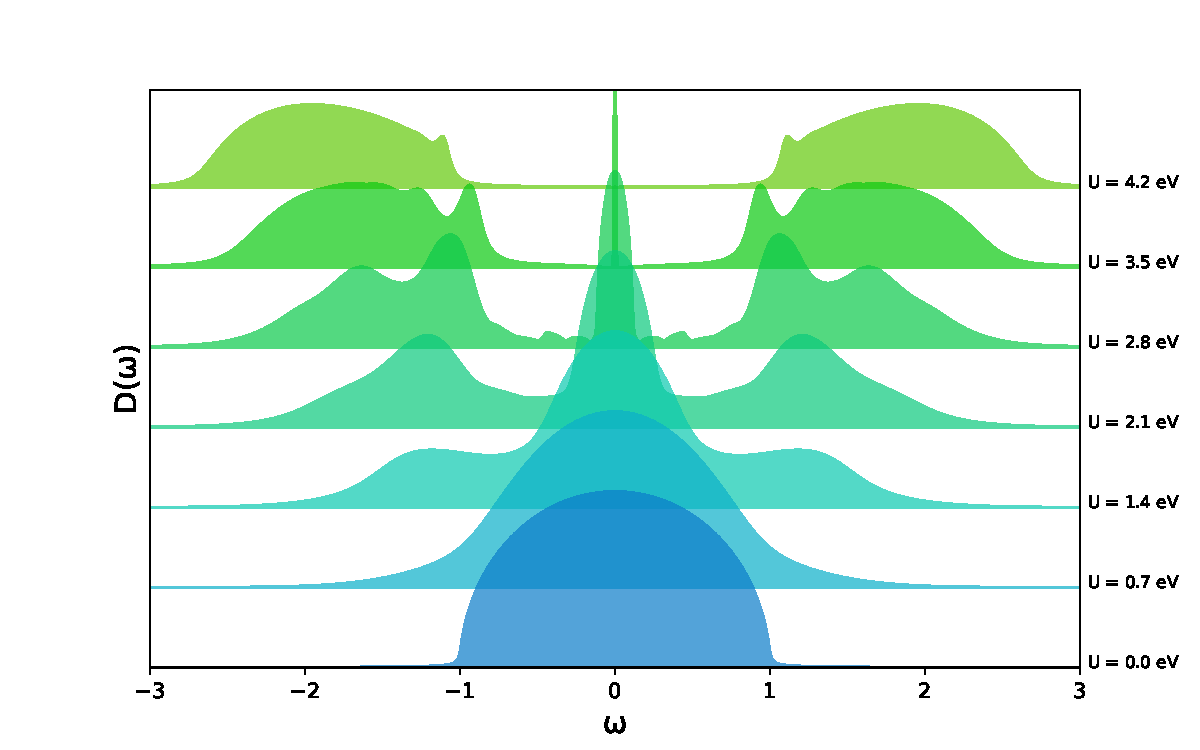
\includegraphics[width=1.00\textwidth]
		{pics/evolUDOS_IPT.pdf}
	\includegraphics[width=1.00\textwidth]
		{pics/evolUΣ2_IPT.pdf}
		\caption{(Atas) Evolusi DOS terhadap interaksi lokal $U$, dan (Bawah) Evolusi dari nilai imajiner \textit{self-energy} dari variasi $U$ yang sama pada temperatur $T = 0 K$ dengan menggunakan metode penyelesaian impuritas teori iterasi pertubasi (IPT)}
\end{figure}	

Transisi logam-isolator juga dipengaruhi oleh temperatur. Gambar 4.2 memperlihatkan evolusi DOS dan \textit{self-energy} dari perhitungan IPT terhadap variasi temperatur dengan interaksi $U = 2.4$ eV. Kami mencacah temperatur pada interval yang sempit untuk melihat transisi secara jelas. Diperlihatkan terjadi transisi fasa dari logam ke isolator secara tiba-tiba pada temperatur sekitar $T = 357 K$. Ini juga diperlihatkan dari perilaku \textit{self-energy}, dimana pada terjadinya transisi, terjadi perubahan dua puncak disekitar energi fermi $\omega = 0$, menjadi satu puncak tepat pada energi fermi $\omega = 0$, hal ini mengakibatkan isolasi elektron pada satu kisi saja akibat interaksi antar elektron.
\begin{figure}
	\centering
	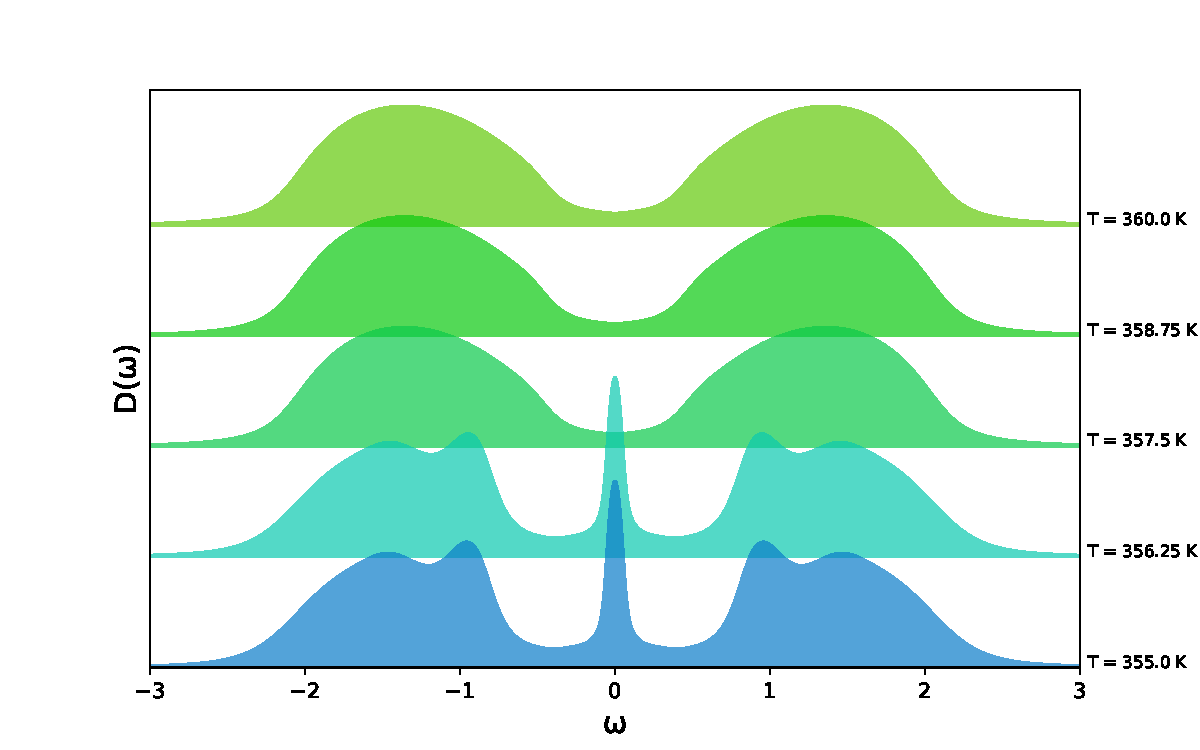
\includegraphics[width=1.00\textwidth]
		{pics/evolTDOS_IPT.pdf}
	\includegraphics[width=1.00\textwidth]
		{pics/evolTΣ2_IPT.pdf}
		\caption{(Atas) Evolusi DOS terhadap temperatur $T$, dan (Bawah) Evolusi dari nilai imajiner \textit{self-energy} dari variasi $T$ yang sama pada $U = 2.4$ dengan menggunakan metode penyelesaian impuritas teori iterasi pertubasi (IPT)}
\end{figure}	

Fase diagram paramagnetik yang dihitung dengan iterasi pertubasi teori ditunjukkan oleh gambar 4.3. Hasil yang diperoleh telah sesuai dengan literatur yang dihitung dengan metode penyelesaian yang lebih eksak seperti quantum monte-carlo\cite{ctqmc}. Hal ini dikarenakan IPT atau koreksi diagram hingga orde sudah cukup mampu untuk menyelesaikan kasus sistem material pada dimensi cenderung tinggi, dan pada kasus \textit{half-filling} dengan menampakkan perilaku transisi logam-isolator. Kita perhatikan bahwa, terdapat daerah ko-eksistensi logam-isolator dibawah parameter kritis $U_c,T_c$.  Koeksistensi mengisyaratkan masih terdapat adanya puncak eksitasi quasipartikel pada $\omega = 0$ dalam parameter tersebut, namun tidak sepenuhnya logam yang baik, dikarenakan jumlah keadaan quasipartikel sangat terbatas pada rentang energi tertentu saja.
\begin{figure}
	\centering
	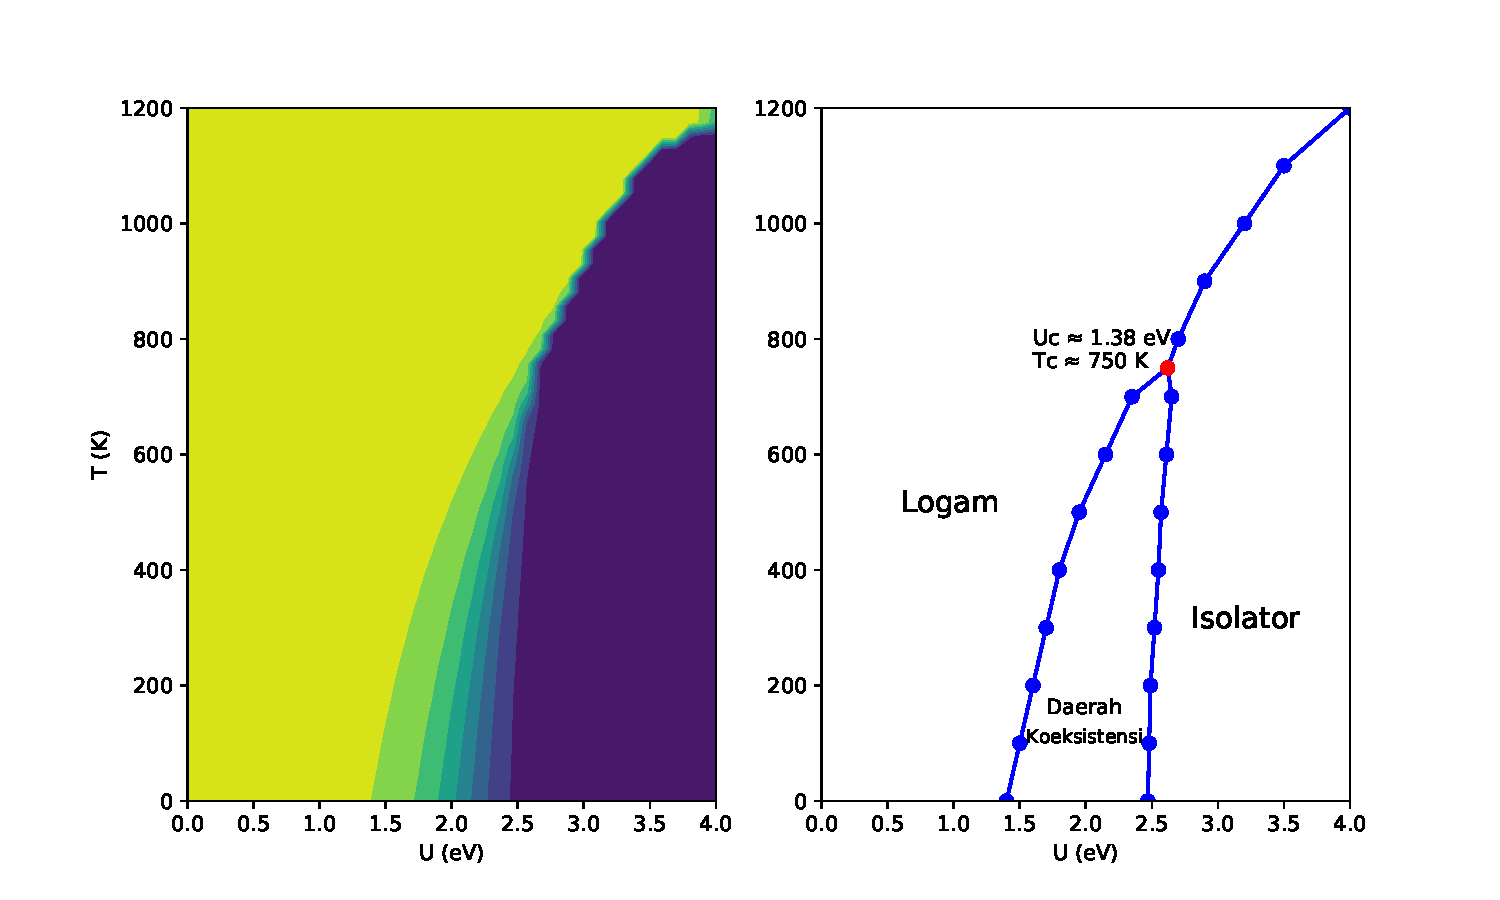
\includegraphics[width=1.00\textwidth]
		{pics/ipt_ph_diagram_param.pdf}
		\caption{Fase diagram paramagnetik transisi logam isolator yang dihitung dengan iterasi pertubasi teori (IPT)}
\end{figure}

Perhitungan pada kasus paramagnetik juga dilakukan untuk metode penyelesaian impuritas fluktuasi okupansi. Hal ini dilakukan untuk melihat perilaku \textit{self-energy} yang dihasilkan oleh fluktuasi okupansi. Evolusi DOS dan imajiner \textit{self-energy} diperlihatkan oleh gambar 4.4. Dengan memaksa sistem untuk berperilaku paramagnetik, melainkan okupnasi untuk kedua basis $\left\lbrace\uparrow,\downarrow\right\rbrace$ dipaksa sama, maka fluktuasi okupansi yang diberikan pada dasarnya tidak berpengaruh apa-apa. Hal ini dapat dikatakan karena jika kita mengidentifikasi fluktuasi dari probabilitas okupansi yang dihitung pada persamaan (3.32), yang diperlihatkan oleh gambar 4.5, terjadi simetrisasi antara nilai maksimum dan minimum, begitu juga untuk okupansi pada kedua basis $\left\lbrace\uparrow,\downarrow\right\rbrace$. Dengan menggunakan probabilitas okupansi yang simetri untuk kedua basis, sebagai perata-rataan fungsi Green yang dihitung pada persamaan (3.34), maka tidak heran jika fluktuasi okupansi ini pada dasarnya memberikan nilai rata-rata nol, atau mendekati nol. Pada kasus paramagnetik, hal ini memberikan kasus yang tak jauh berbeda dengan pendekatan medan rata-rata biasa.
\begin{figure}
	\centering
	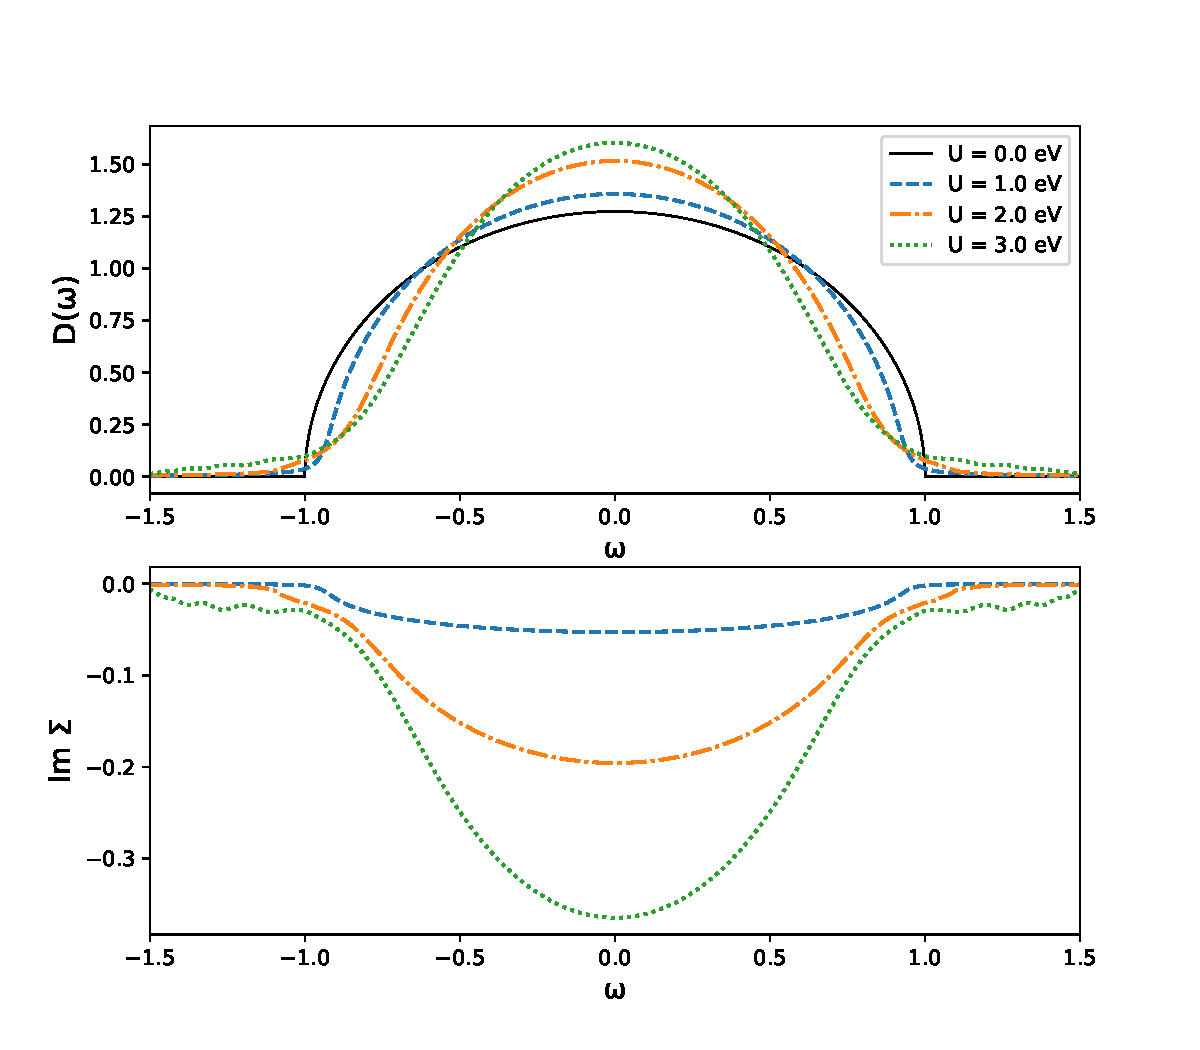
\includegraphics[width=1.00\textwidth]
		{pics/evolUDOS_OF.pdf}
		\caption{Evolusi DOS dan $\text{Im}\Sigma$ dari metode fluktuasi okupansi pada temperatur rendah $T = 50K$.}
	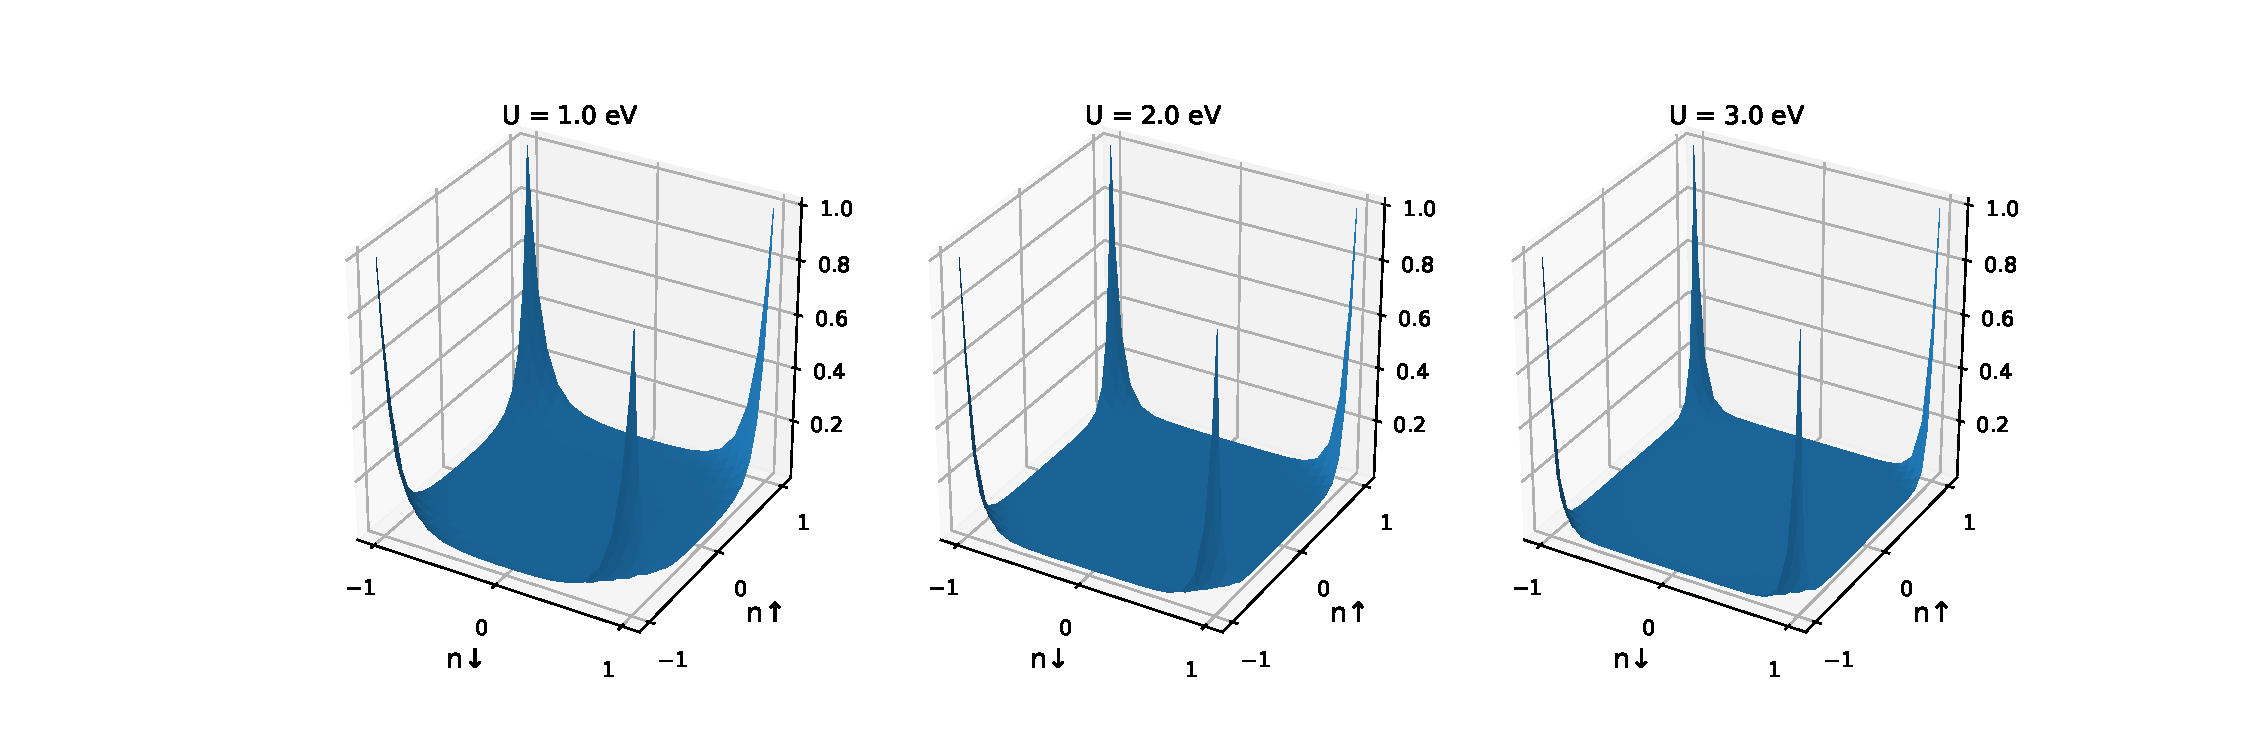
\includegraphics[width=1.00\textwidth]
		{pics/evolUProbabs_OF_PM.pdf}
		\caption{Probabilitas fluktuasi untuk kedua basis $\left\lbrace \uparrow, \downarrow \right\rbrace$ pada temperatur rendah $T = 50K$, dengan tiga variasi interaksi $U$.}
\end{figure}

Walaupun begitu, terlihat \textit{self-energy} tidak bernilai nol. Jika dilihat perilaku \textit{self-energy}, kurvanya menunjukkan seperti kurva semi-lingkaran seperti yang diperoleh dari kisi bethe. Hal ini bisa dipahami karena persamaan \textit{self-energy} didapat dari persamaan (3.35) sepenuhnya berasal dari informasi fungsi Green, baik impuritas maupun fungsi green kolam yang dua kuantitas itu sangat erat mengandung informasi kisi bethe. Hal ini juga diperkuat dengan hasil perata-rataan fungsi Green dari fluktuasi yang simetri sehingga kembali yang pada nilai yang tidak jauh berbeda dari nilai awal sebelum diberi fluktuasi. 
\begin{align}
G_{\text{ave}}(i\omega_n) \approx G_0(i\omega_n)
\end{align}
Perilaku \textit{self-energy} ini masih belum dapat diterima sebagai hasil fisis yang baik seperti halnya IPT yang didapat dari diagram orde-2. Okupansi fluktuasi sebagai metode penyelesaian impuritas pada kasus paramagnetik masih belum memberikan hasil yang memuaskan. 

%-----------------------------------------------------------------------------%
\section{Keadaan Antiferromagnetik}
%-----------------------------------------------------------------------------%
Terdapat keadaan dasar lain pada \textit{half-filling} yakni antiferomagnetik. Pada kalkulasi antiferomagnetik, orde satu diagram \textit{self-energy} atau perhitungan okupansi diperhitungkan. Perhitungan okupansi ini dilakukan di semua metode penyelesaian impuritas. Gambar 4.6 memperlihatkan total DOS dan DOS dari masing-masing basis $\text{Im} \Sigma$, untuk metode penyelesaian medan rata-rata. 

Gambar 4.6 memperlihatkan bahwa kedua spin memiliki jumlah keadaan energi yang saling berlawanan, hal ini akibat perbedaan nilai spin yang saling berlawanan. Dari sini terlihat pula, setiap spin memiliki DOS yang menyerupai DOS untuk kisi FCC. Hal tersebut dapat dijelaskan dengan bahwa setiap keadaan spin menempati satu sub-kisi (A) dan spin lain menempati sub kisi lain (B). Sehingga, pada kisi kubik, sub-sub kisi ini saling membentuk kisi FCC antara sub-kisi sejenisnya, sehingga tentu setiap spin memiliki bentuk DOS yang serupa. Namun terdapat bagian dari DOS dari masing-masing spin menempatin daerah energi berlawanan, hal ini dapat dijelaskan jika kita masih melihat elektron sebagai densitas fungsi gelombang, pada $U$ yang relatif rendah, densitas elektron masih berada sub kisi A dan sub kisi B, dengan densitas yang berbeda. Perilaku \textit{self-energy} sepenuhnya tidak bergantung dengan energi $\omega$, dimana bernilai konstan, dan memiliki nilai yang berlawanan antara \textit{self-energy} untuk basis $\left\lbrace\uparrow\right\rbrace$ dan basis $\left\lbrace\downarrow\right\rbrace$.
\begin{figure}
	\centering
	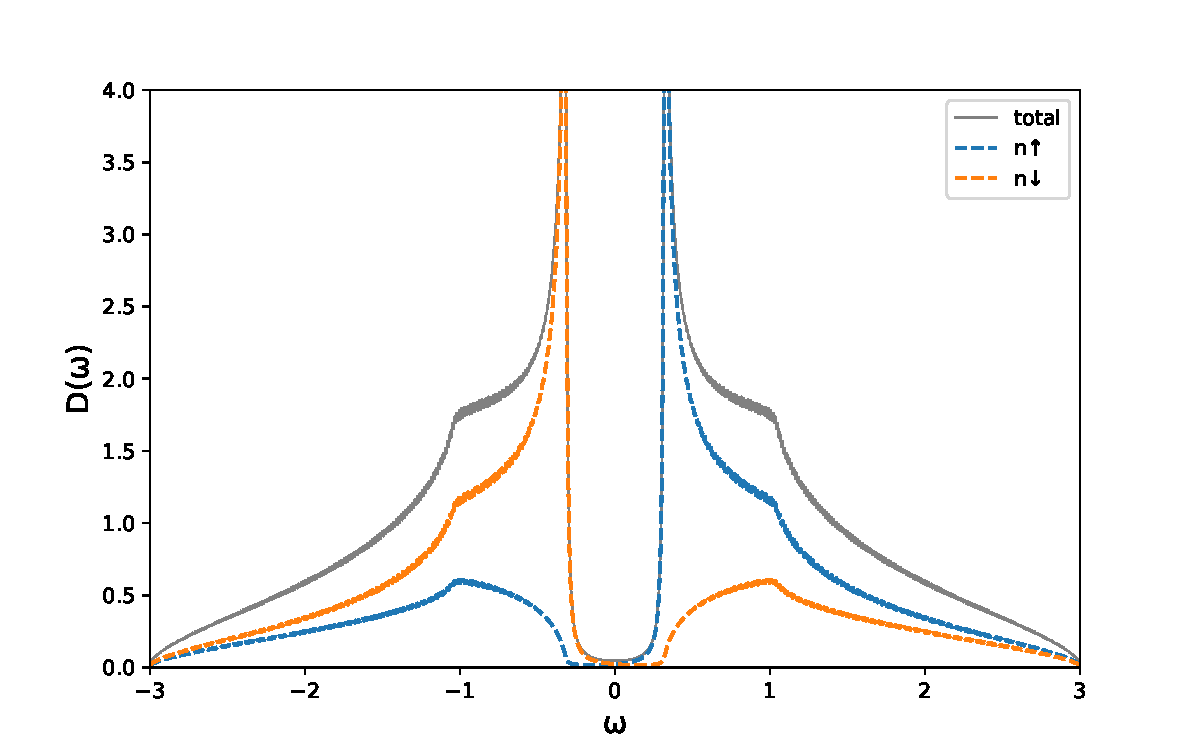
\includegraphics[height=0.5\textwidth, width=1.0\textwidth]
		{pics/dosupdown_MF_AF.pdf}
		\caption{Evolusi DOS terhadap $U$ pada temperatur $T = 0 K$ dan evolusi DOS terhadap $T$ pada $U = 1.5 eV$}
\end{figure}

Berikut juga diperlihatkan Gambar 4.7 evolusi DOS terhadap $U$ dan Temperatur $T$ dari perhitungan medan rata-rata. Formasi Gap sepenuhnya berasal dari perbedaan okupansi, dan pengaruh temperatur mengakibat besarnya eksitasi termal.
\begin{figure}
	\centering
	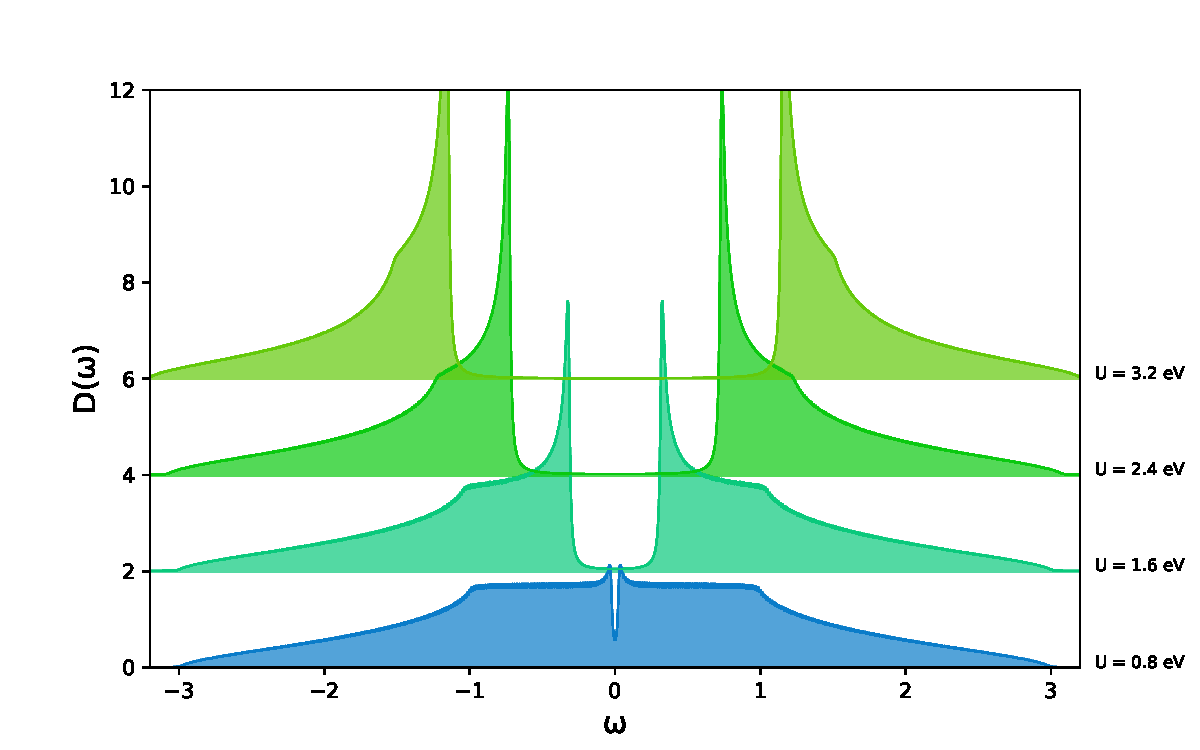
\includegraphics[height=0.4\textwidth, width=1.0\textwidth]
		{pics/evolUDOS_MF_AF.pdf}
	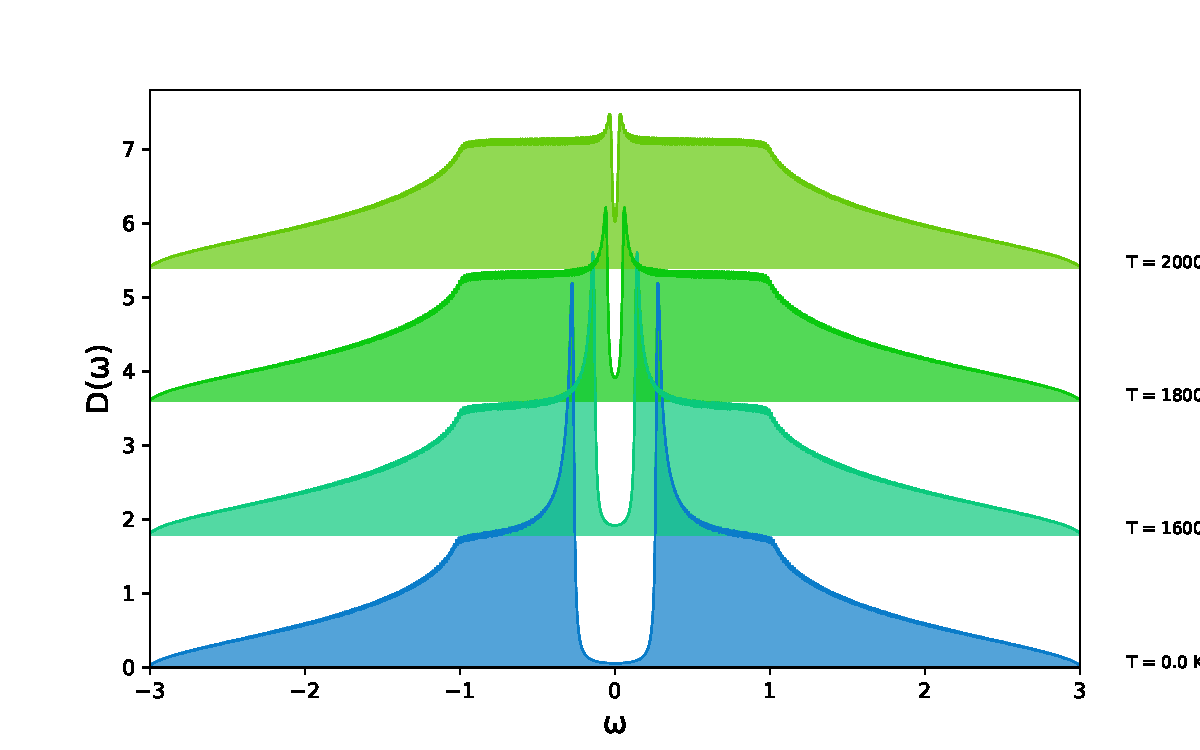
\includegraphics[height=0.4\textwidth, width=1.0\textwidth]
		{pics/evolTDOS_MF_AF.pdf}
		\caption{DOS dan DOS dari masing-masing basis orbital dengan perhitungan medan rata-rata, pada $U = 1.6 eV$ dan $T = 0.0 K$}
\end{figure}

Gambar 4.8 memperlihatkan perhitungan DOS melalui metode penyelesaian impuritas $IPT$ dengan $U = 2.0$ dan temperatur $T = 150 K$, DOS dua basis juga memiliki perilaku yang sama, namun sudah tidak sepenuhnya membentuk DOS FCC. Hal ini dikarenakan terdapat kontribusi diagram orde 2 pada \textit{self-energy}-nya. Pita DOS basis pada daerah energi berlawanannya (rentang energi negatif untuk basis $\uparrow$ dan positif untuk basis $\downarrow$) cenderung untuk menyebar. Hal ini bisa jika lihat pada $\text{Im}\Sigma$ yang memiliki dua puncak pada daerah energi relatif cukup tinggi, namun amplitudonya relatif kecil, yang mengindikasikan masih adanya kecendrungan untuk menyebar pada daerah energi tinggi, dan gap dari pita terbentuk berasal dari kontribusi diagram orde satu, atau nilai okupansi kedua basis dilihat perbedaan amplitudo dari $\text{Re}\Sigma$.
\begin{figure}
	\centering
	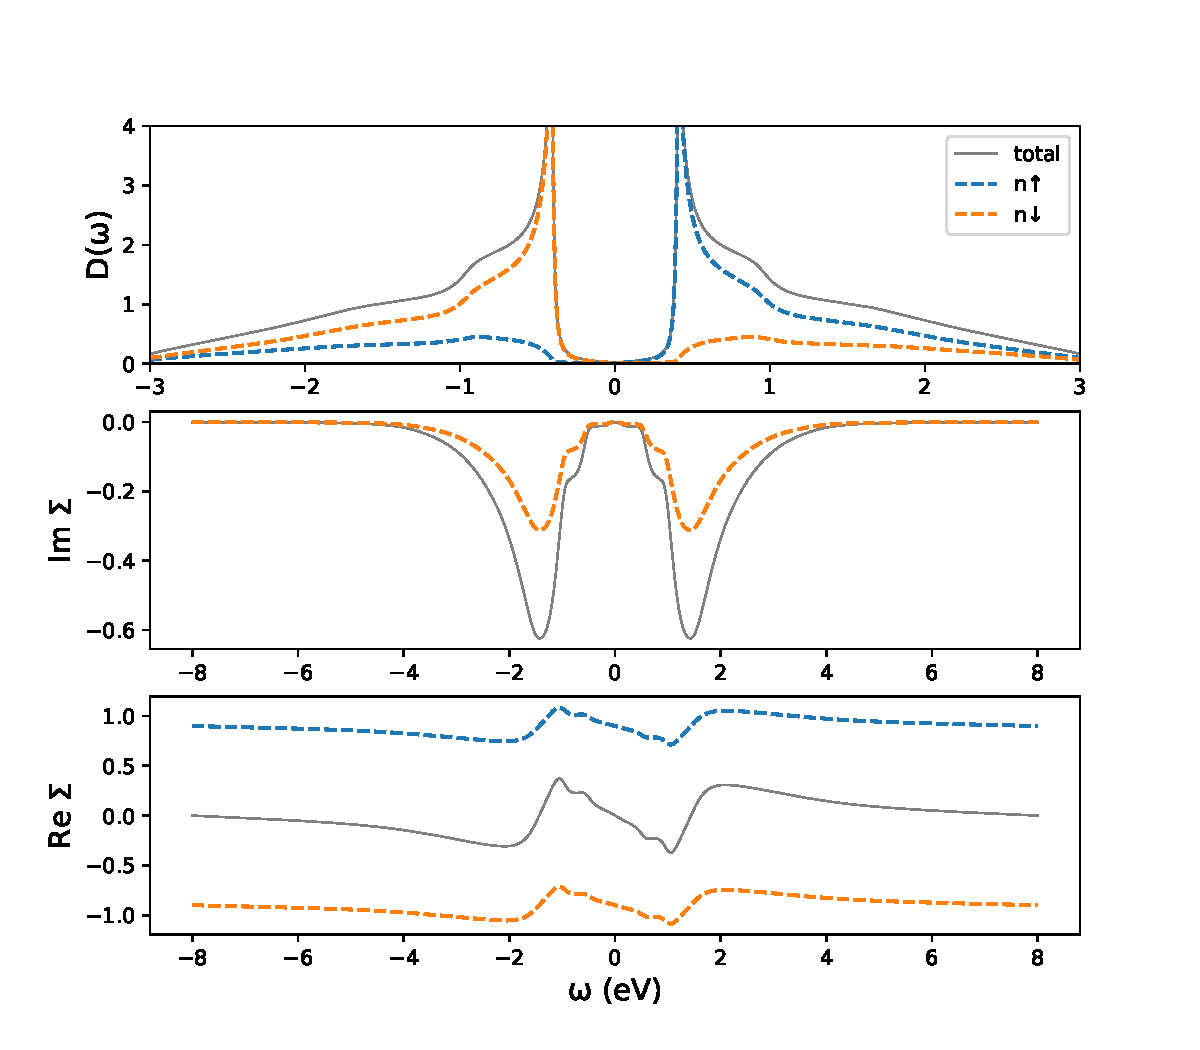
\includegraphics[width=1.0\textwidth]
		{pics/dosupdown_IPT_AF.pdf}
		\caption{DOS dan DOS dari masing-masing basis orbital dengan perhitungan IPT, pada $U = 2.0 eV$ dan $T = 150 K$}
\end{figure}

Selanjutnya, masih dalam IPT, kita lihat evolusi DOS untuk variasi interaksi lokal $U$. Evolusi DOS beserta $\textit{Im}\Sigma$ tersebut diperlihatknan pada gambar 4.9.
\begin{figure}
	\centering
	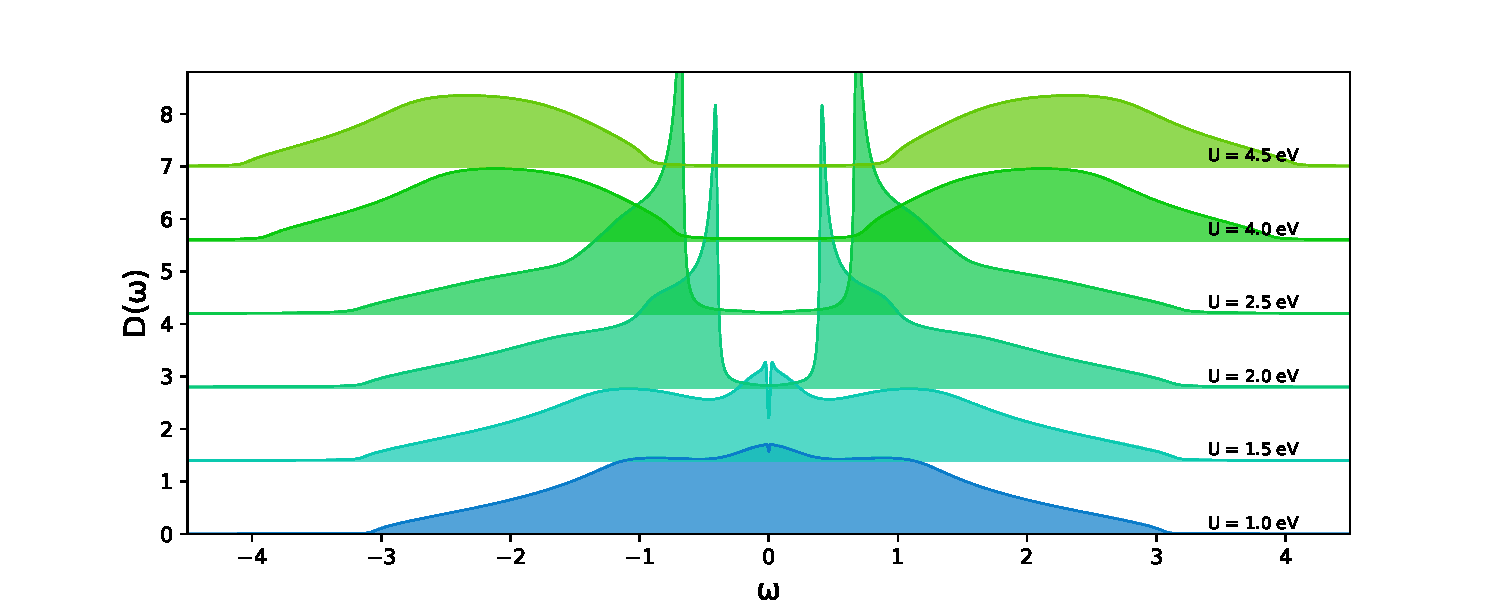
\includegraphics[width=1.0\textwidth]
		{pics/evolUDOS_IPT_AF.pdf}
	\includegraphics[width=1.0\textwidth]
		{pics/evolUΣ2_IPT_AF.pdf}
		\caption{Evolusi DOS dan nilai $\text{Im}\Sigma$ nya terhadap variasi $U$ pada temperatur $T = 150K$ menggunakan metode penyelesaian impuritas IPT}
\end{figure}

Pada $U$ yang relatif rendah, terdapat formasi quasipartikel, dan dalam hal ini okupansi untuk kedua basis masih relatif sama. Nilai $\text{Im}\Sigma$ menunjukkan alasan mengapa terjadi formasi quasipartikel sama halnya dengan kasus paramagnetik. Pada $U$ selanjutnya, formasi gap terjadi, dan ini berasal dari perbedaan nilai okupansi spin antara kedua kisi, dan puncak quasipartikel tidak lagi dapat dilihat akibat pengaruh formasi gap ini, namun dari nilai $\text{Im}\Sigma$ masih mengindikasikan seharusnya terdapat pita quasipartikel pada daerah energi fermi. Sedangkan pada $U$ yang tinggi, formasi gap tidak berasal dari perbedaan okupansi, melainkan kontribusi dari \textit{self-energy}, dimana dapat kita lihat nilai $\text{Im}\Sigma$ memiliki amplitudo yang sangat tinggi pada daerah energi fermi, yang kembali mengindikasikan tingginya energi interaksi pada energi rendah sehingga mengakibatkan lokalisasi.

Jika kita selanjutnya kita melihat evolusi DOS dengan variasi temperatur $T$, yang diperlihatkan oleh gambar 4.10. Formasi gap hilang dikarenakan berasal dari fluktuasi termal yang tinggi. Sedangkan jika dilihat dari kontribusi \textit{self-energy} orde dua, perubahan terjadi secara kontinu, dan memberikan formasi quasipartikel disaat hilangnya gap. Terjadi kompetisi quasipartikel dan perbedaan okupansi, pada temperatur transisi, ini mengakibatkan transisi secara mendadak pada keberadaan gap.
\begin{figure}
	\centering
	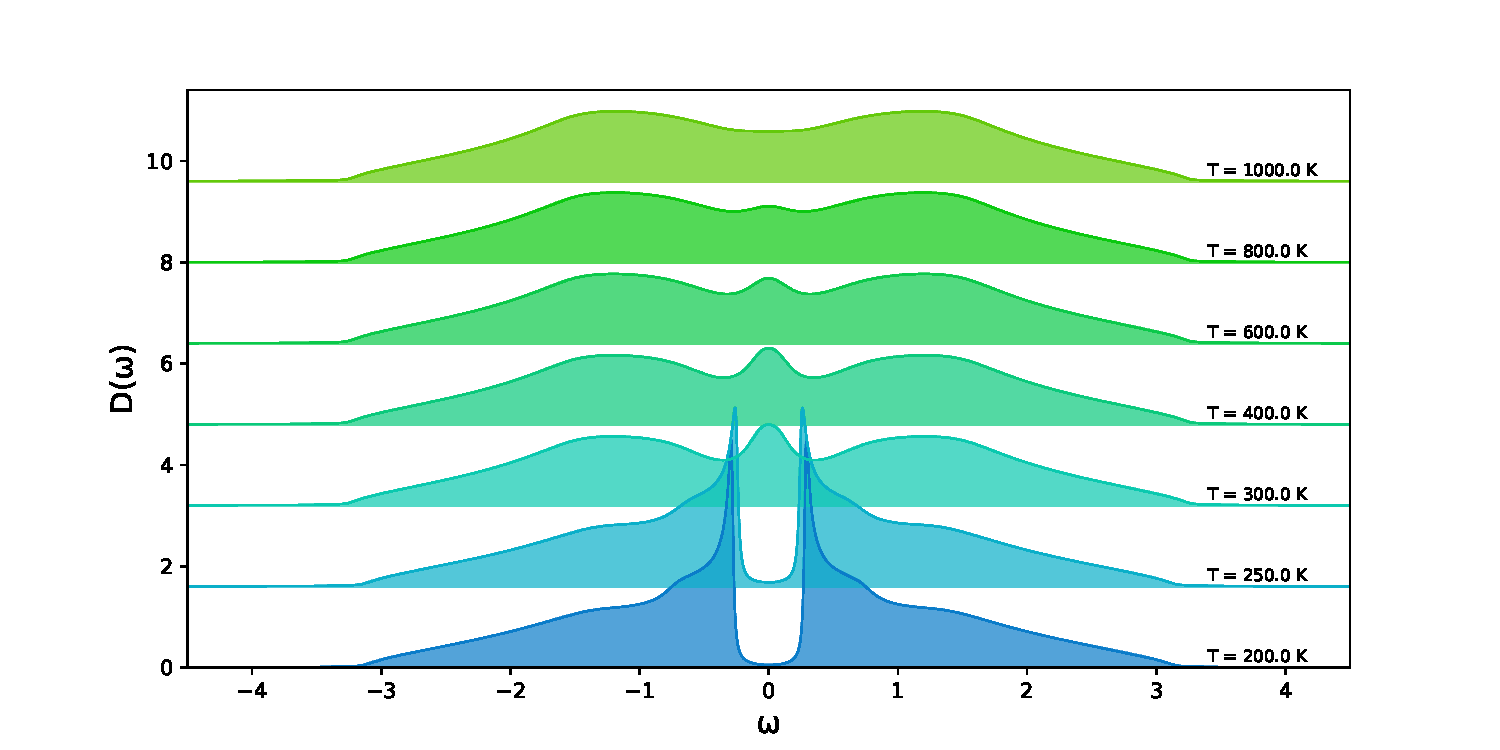
\includegraphics[width=1.0\textwidth]
		{pics/evolTDOS_IPT_AF.pdf}
	\includegraphics[height=0.4\textwidth, width=1.0\textwidth]
		{pics/evolTΣ2_IPT_AF.pdf}
		\caption{Evolusi DOS dan nilai $\text{Im}\Sigma$ nya terhadap variasi $T$ pada temperatur $U = 1.8$ eV menggunakan metode penyelesaian impuritas IPT}
\end{figure}

Pada perhitungan menggunakan okupansi fluktuasi murni, jika kita melihat DOS dan DOS masing-masing dari basis yang diperlihatkan gambar 4.11. Terlihat pada gambar tersebut dua puncak kecil pada daerah gap. Hal ini dapat kita lihat penyebabnya berasal dari $\Sigma$ yang semata-mata tidak hanya berasal dari kontribusi perbedaan okupansi, tetapi juga fluktuasinya. Tidak seperti halnya IPT yang seragam untuk kedua basis, nilai $\text{Im}\Sigma$ masing-masing memberikan nilai yang berbeda untuk kedua basis, hal ini wajar dikarenakan fluktuasi kedua basis memberikan nilai yang saling berlawanan. Fitur ini tentu tidak dimiliki oleh medan rata-rata biasa yang sama sekali menghilangkan fluktuasi okupansi didalamnya.

Evolusi DOS terhadap $U$ yang ditunjukkan oleh gambar 4.12 memperlihatkan pada $U$ yang rendah, terjadi paramagnetisme, yang kembali nilai $\text{Im}\Sigma$ merupakan bentuk yang sama dengan DOS dari kubik, sehingga pada $U$ yang rendah, belum dapat diterima secara fisis. Namun pada $U$ yang tinggi, dimana terjadi perbedaan okupansi yang berarti, nilai $\text{Im}\Sigma$ memberikan puncak-puncak tajam yang mengindikasi adanya fluktuasi interaksi elektron-elektron didalamnya.
\begin{figure}
	\centering
	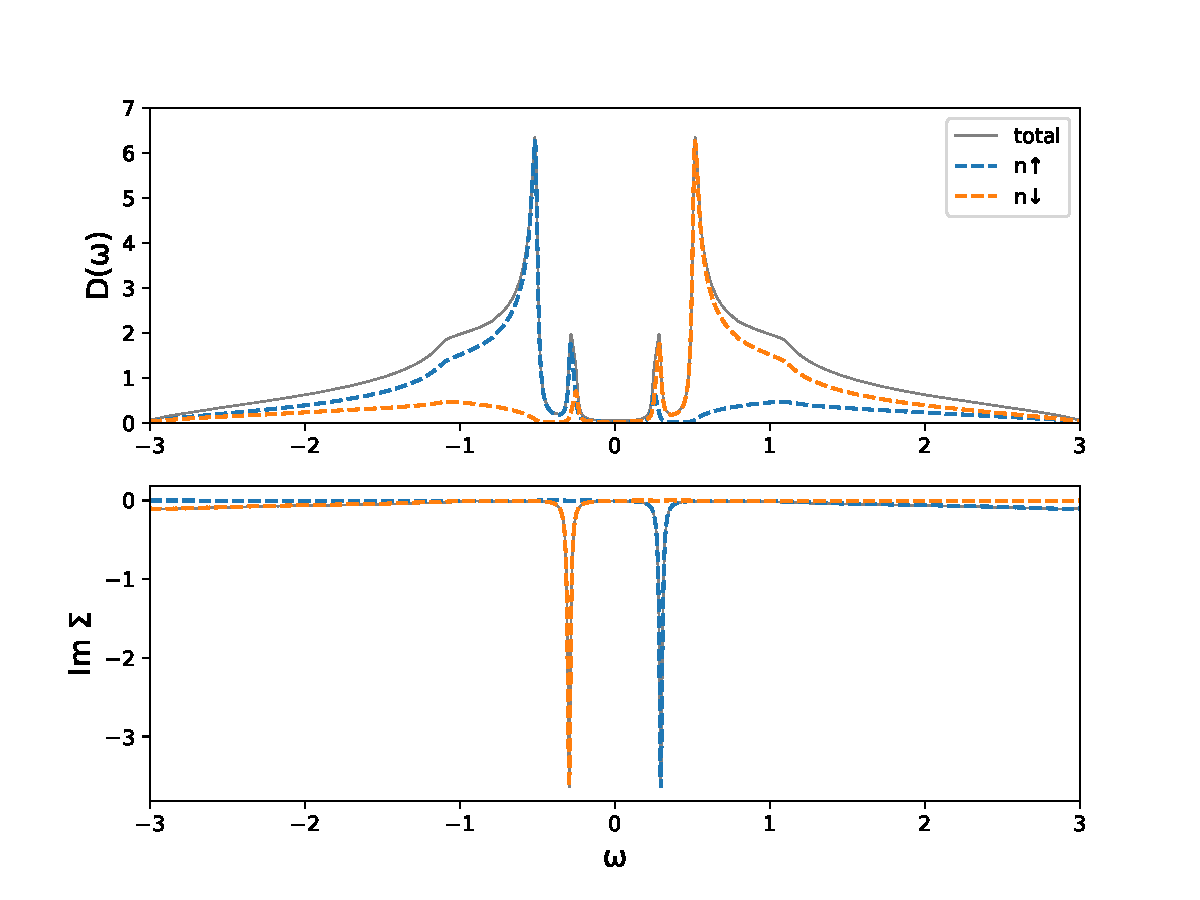
\includegraphics[width=0.9\textwidth]
		{pics/dosupdown_OF_AF.pdf}
		\caption{DOS dan DOS dari masing-masing basis orbital dengan perhitungan fluktuasi okupansi, pada $U = 2.0 eV$ dan $T = 20 K$}
\end{figure}

\begin{figure}
	\centering
	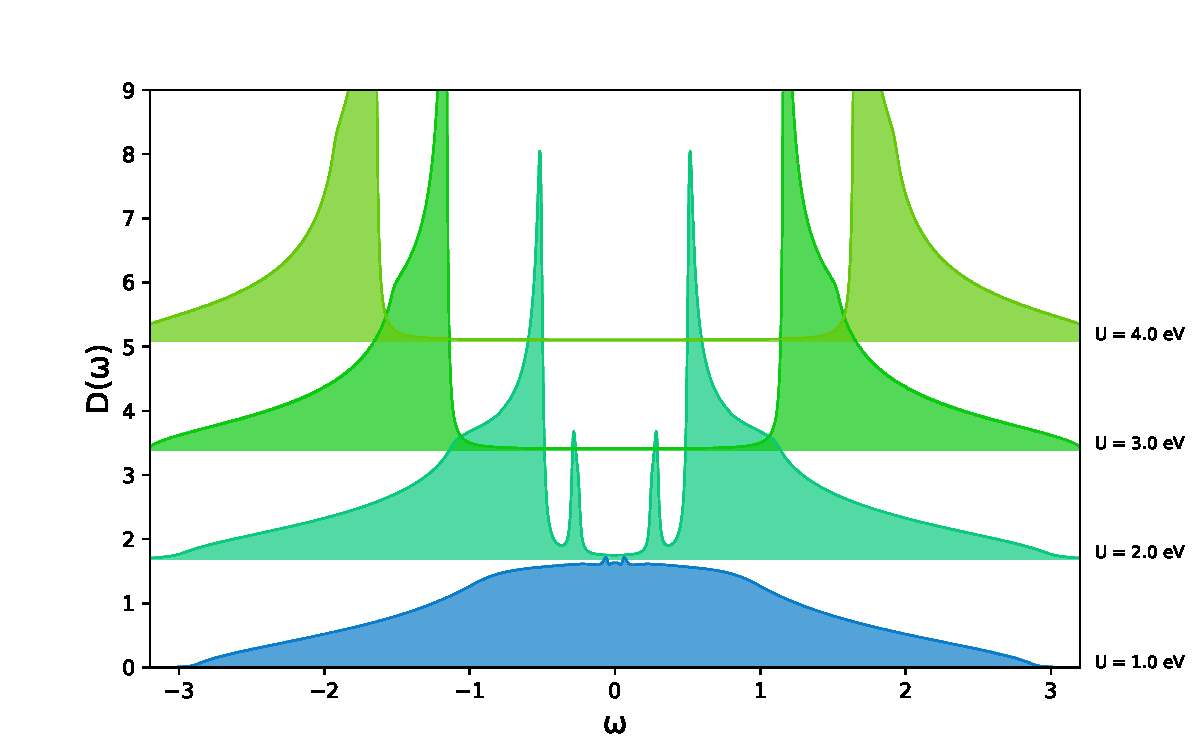
\includegraphics[height=0.4\textwidth, width=1.0\textwidth]
		{pics/evolUDOS_OF_AF.pdf}
	\includegraphics[height=0.35\textwidth, width=1.0\textwidth]
		{pics/evolUΣ_OF_AF.pdf}
		\caption{Evolusi DOS dan nilai $\text{Im}\Sigma$ nya terhadap variasi $T$ pada temperatur $U = 1.8$ eV menggunakan metode penyelesaian impuritas IPT}
\end{figure}

Selanjutnya evolusi DOS dan $\text{Im}\Sigma$ terhadap temperatur ditunjukkan oleh gambar 4.13. Hilangnya formasi gap dikarenakan fluktuasi termal, dan juga tingginya fluktuasi okupansi. Dapat kita lihat, kembali pada daerah paramagnetik, nilai $\text{Im}\Sigma$ membentuk nilai informasi yang sama dengan DOS paad kubik dengan nilai $U$ yang terbatas. Dapat dipastikan, segala keadaan paramagnetik pada okupansi fluktuasi, kurang memberikan hasil fisis yang tepat sebagai metode penyelesaian impuritas untuk DMFT.
\begin{figure}
	\centering
	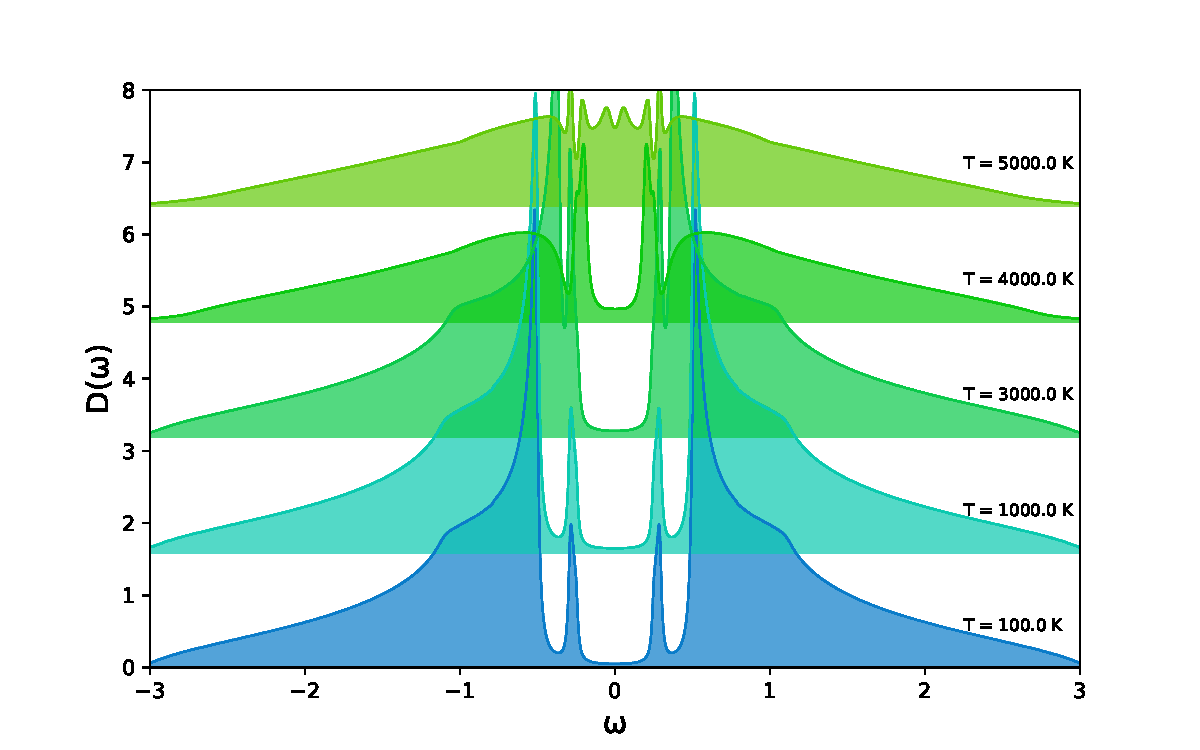
\includegraphics[height=0.4\textwidth, width=1.0\textwidth]
		{pics/evolTDOS_OF_AF.pdf}
	\includegraphics[height=0.35\textwidth, width=1.0\textwidth]
		{pics/evolTΣ_OF_AF.pdf}
		\caption{Evolusi DOS dan nilai $\text{Im}\Sigma$ nya terhadap variasi $T$ pada temperatur $U = 1.8$ eV menggunakan metode penyelesaian impuritas IPT}
\end{figure}

\subsection{Okupansi Fluktuasi sebagai Koreksi IPT}
Dari hasil keadaan paramagnetik tersebut, kami termotivasi untuk menjadi okupansi fluktuasi bukan sebagai metode penyelesaian impuritas DMFT yang utama, melainkan sebagai koreksi okupansi dari IPT, selanjutnya akan disebut sebagai IPT+OF. Perhitungan dilakukan sesuai diagram algoritma yang dijelaskan pada bab 3, dimana hasil dari IPT digunakan sebagai nilai masukan untuk okupansi fluktuasi. 

Gambar 4.14 memperlihatkan DOS total dan DOS untuk kedua basis, serta nilai $\text{Im}\Sigma$ pada $U$ yang relatif tinggi yakni $U = 4.0$ eV. Dapat kita lihat bahwa informasi DOS mengisyaratkan bahwa sistem belum menjadi paramagnetik, melainkan antiferomagnetik, tetapi bentuk kurvanya berbeda dari antiferomagnetik yang ditunjukkan oleh DOS yang hanya akibat perbedaan okupansi. Nilai $\text{Im}\Sigma$ juga memberikan perbedaan \textit{shift} untuk kedua basis yang berbeda, dimana tidak sepenuhnya bernilai sama seperti yang didapat dari IPT. Dari IPT kita lihat bahwa gap terbentuk akibat kompetisi perbedaan okupansi dan kuatnya interaksi pada energi rendah, namun pada IPT+OF gap dapat terjadi akibat koeksistensi dari perbedaan okupansi dan koreksi 
\textit{self-energy} diagram orde dua. Hilangnya karakter gap yang hanya dikarenakan perbedaan okupansi juga disebabkan oleh fluktuasi termal dimana pada gambar 4.14 nilai temperatur $T = 150K$.
\begin{figure}
	\centering
	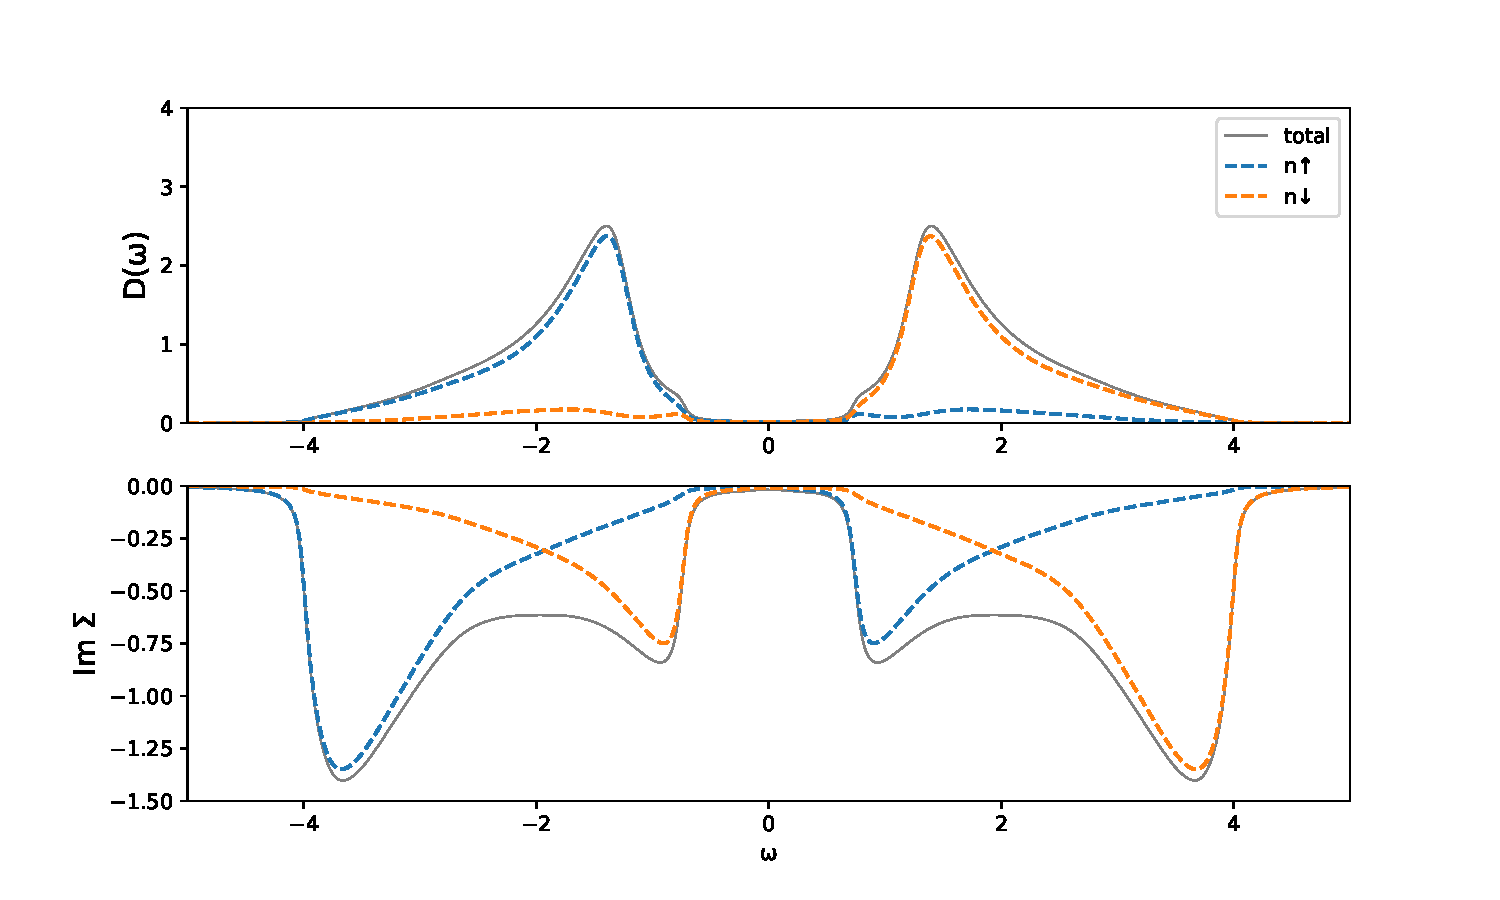
\includegraphics[width=1.0\textwidth]
		{pics/dosupdown_OFIPT_AF.pdf}
		\caption{DOS dan DOS dari masing-masing basis orbital dengan perhitungan IPT+OF, pada $U = 4.0 eV$ dan $T = 150K K$}
\end{figure}

Gambar 4.15 memperlihatkan evolusi DOS dan $\text{Im}\Sigma$ dari IPT+OF terhadap $U$, dimana pada $U$ yang relatif tinggi, sistem masih mempertahankan sifat antiferomagnetismenya walaupun kondisi fisis sudah berbeda dari antiferomagnetisme akibat perbedaan okupansi biasa. Jika dilihat perilaku $\text{Im}\Sigma$, pada $U$ relatif rendah, ini memiliki kontribusi seperti dari yang diberikan oleh OF, karena kontribusi IPT berada pada rentang amplitudo yang rendah untuk energi yang rendah. Sedangkan, pada $U$ yang tinggi, terjadi koeksistensi keduanya.
\begin{figure}
	\centering
	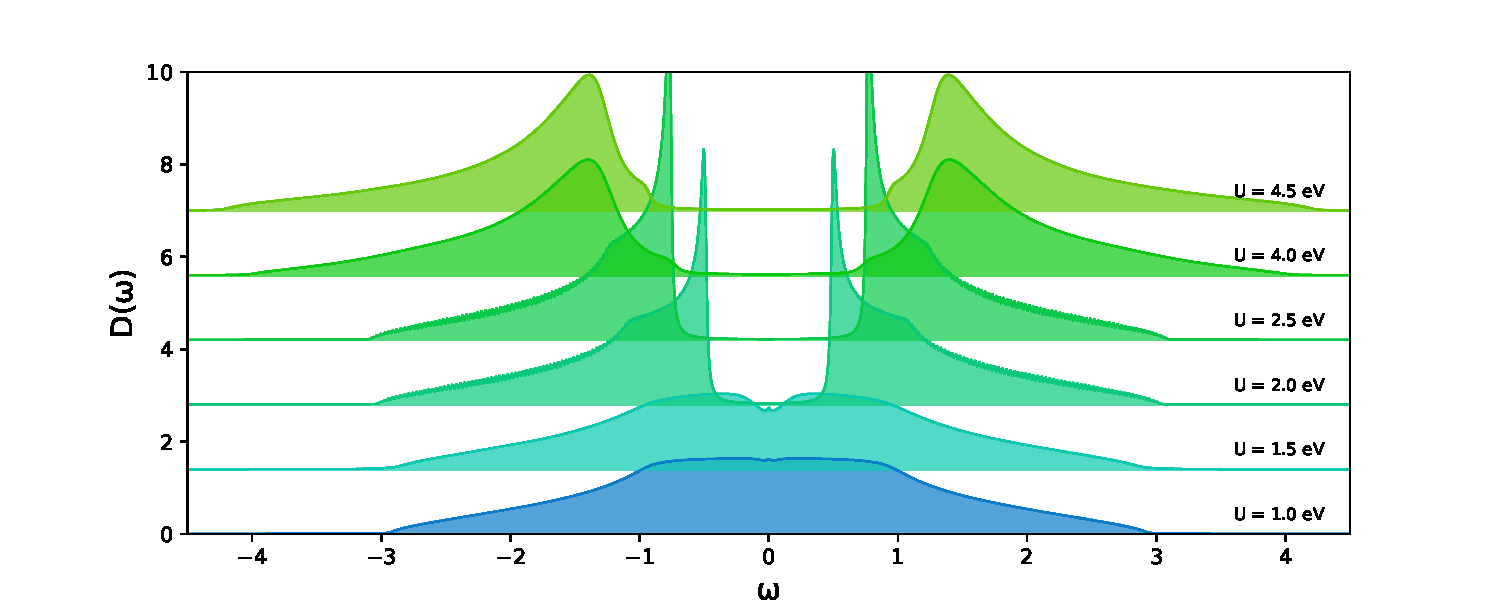
\includegraphics[height=0.4\textwidth, width=1.0\textwidth]
		{pics/evolUDOS_OFIPT_AF.pdf}
	\includegraphics[height=0.35\textwidth, width=1.0\textwidth]
		{pics/evolUΣ2_OFIPT_AF.pdf}
		\caption{Evolusi DOS dan nilai $\text{Im}\Sigma$ nya terhadap variasi $U$ pada temperatur $T = 150 K$ eV menggunakan metode penyelesaian impuritas IPT+OF}
\end{figure}

\begin{figure}
	\centering
	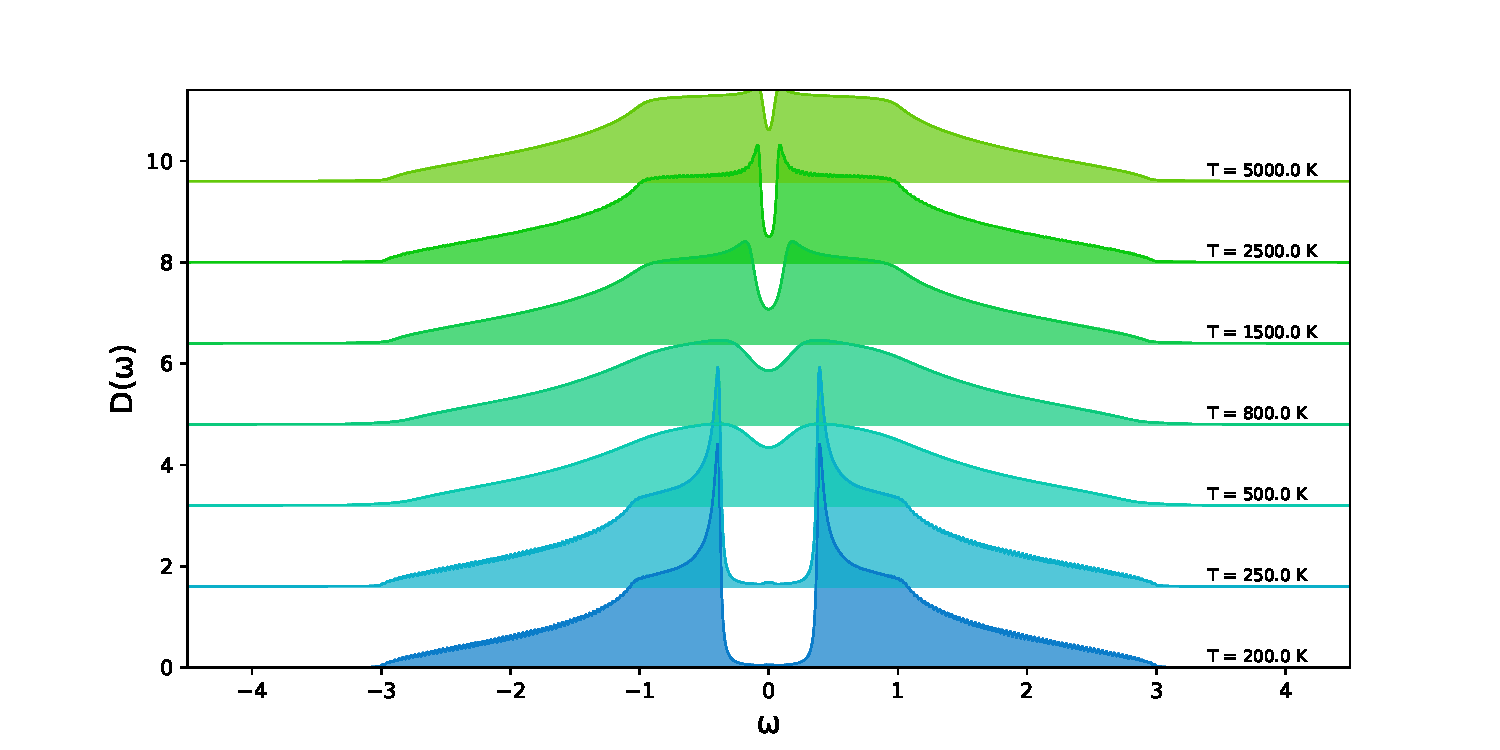
\includegraphics[height=0.4\textwidth, width=1.0\textwidth]
		{pics/evolTDOS_OFIPT_AF.pdf}
	\includegraphics[height=0.3\textwidth, width=1.0\textwidth]
		{pics/evolTΣ2_OFIPT_AF.pdf}
		\caption{Evolusi DOS dan nilai $\text{Im}\Sigma$ nya terhadap variasi $T$ pada temperatur $U = 1.8$ eV menggunakan metode penyelesaian impuritas IPT}
\end{figure}

Gambar 4.16, memperlihatkan evolusi DOS dan $\text{Im}\Sigma$ dari IPT+OF terhadap $T$. Kita lihat bahwa evolusi temperatur pada daerah $T = 200 K$ hingga transisi pada $T = 500K$ merupakan kontribusi dari IPT. Namun, menariknya, pada temperatur yang semakin tinggi, terbentuk pseudogap yang semakin besar, dan kembali tertutup seperti layaknya dari perhitungan medan rata-rata. Hal ini dapat dilihat dari $\text{Im}\Sigma$ yang dimana kontribusi dari OF memiliki peran besar untuk menampilkan perilaku gap DOS sebagai perbedaan okupansi.

Perhitungan IPT+OF memberikan hasil yang menarik, selain memberikan perilaku perbedaan okupansi untuk nilai $\text{Im}\Sigma$, tetapi juga memberikan daerah koeksistensi kontribusi dari gap yang terbentuk akibat perbedaan okupansi dan \textit{self-energy} pada orde kedua. Jika kita melihat perilaku evolusi magnetisme subkisi pada ketiga metode, medan rata-rata, IPT, dan IPT+OF, kita mendapatkan hasil yang menarik, hal ini diperlihatkan pada gambar 4.17. Perubahan pada perhitungan medan rata-rata terjadi secara kontinu, hal ini magnetisme berkolerasi linear terhadap terbentuknya gap, sehingga magnetisme dapat dihitung dengan persamaan gap untuk medan rata-rata\cite{staudt}. Sedangkan pada IPT, akibat koreksi orde 2 dan kompetisinya terhadap perbedaan okupansi, terjadi transisi secara mendadak, baik terhadap perubahan $U$ dan $T$. Selanjutnya pada IPT+OF, dimana fluktuasi okupansi digunakan sebagai koreksi IPT, pada $U$ dan $T$ yang relatif rendah, nilai IPT dan IPT+OF cukup \textit{fitting} satu sama lain, namun terjadinya transisi AF-PM, fluktuasi okupansi berperan menahan terjadinya transisi secara tajam. Akibat adanya fluktuasi okupansi, keadaan PM tidak semerta-merta dapat dicapai dengan mudah.

Hasil utama pekerjaan skripsi ini diperlihatkan dari gambar 4.18. Walaupun dari perilaku magnetisme IPT+OF yang diperlihatkan oleh gambar 4.17, sayangnya diagram fasa magnetisme pada IPT+OF tidak memberikan koreksi yang cukup berarti untuk IPT dalam mengoreksi fasa yang mendekati eksak, yakni $U$ kecil mengikuti persamaan gap dari pendekatan medan rata-rata, dan $U$ yang besar diambil dari batas heisenberg. Perhitungan menggunakan metode penyelesaian impuritas CTQMC\cite{ctqmc} juga diperlihatkan sebagai pembanding, dimana terlihat bahwa metode penyelesaian impuritas menggunakan ctqmc cukup mampu dalam memprediksi diagram fasa kisi kubik pada DMFT, data diambil dari referensi\cite{staudt}.
\begin{figure}
	\centering
	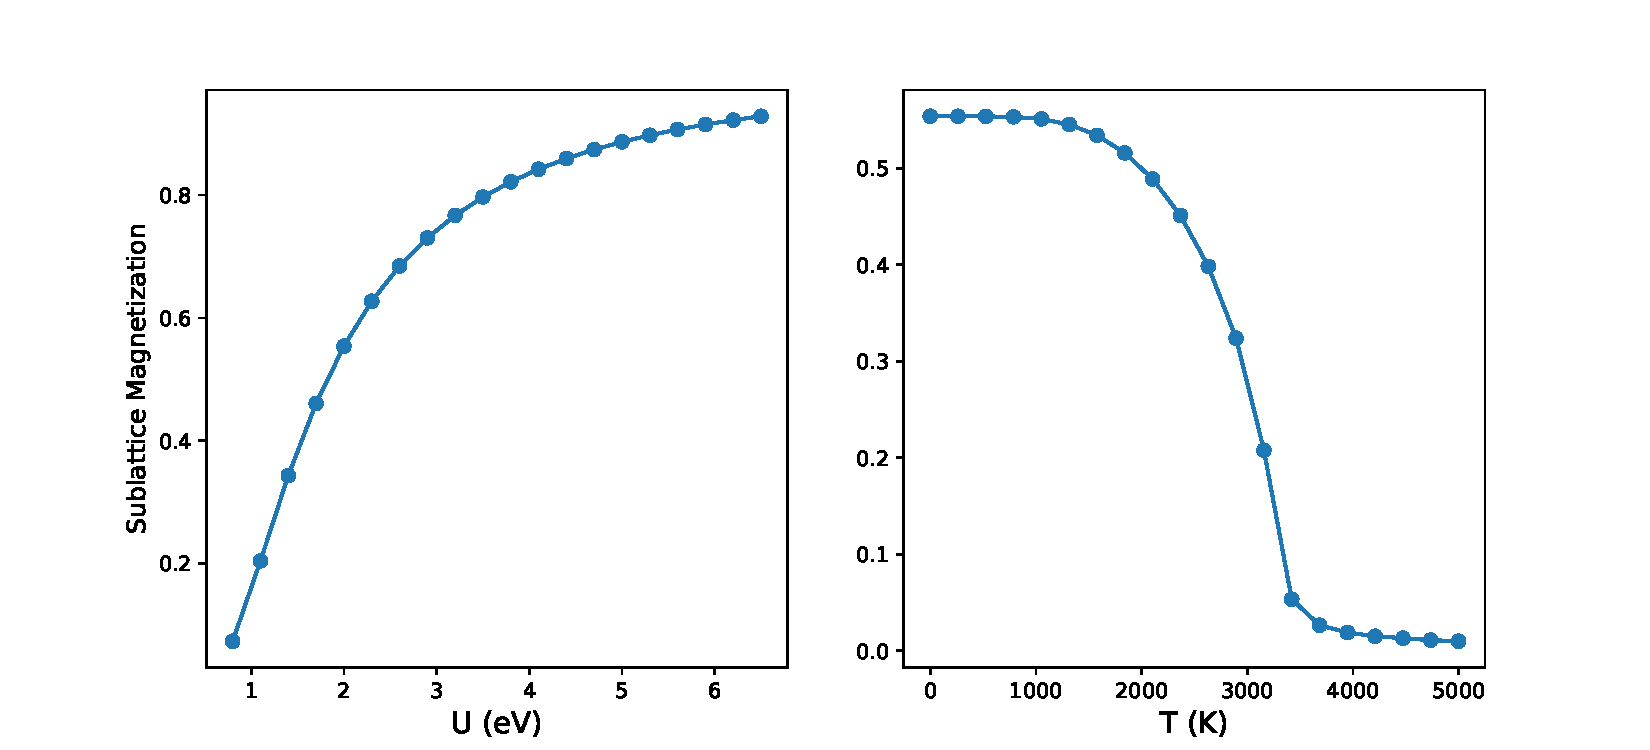
\includegraphics[height=0.5\textwidth, width=1.0\textwidth]
		{pics/magnetization_MF_AF.pdf}
	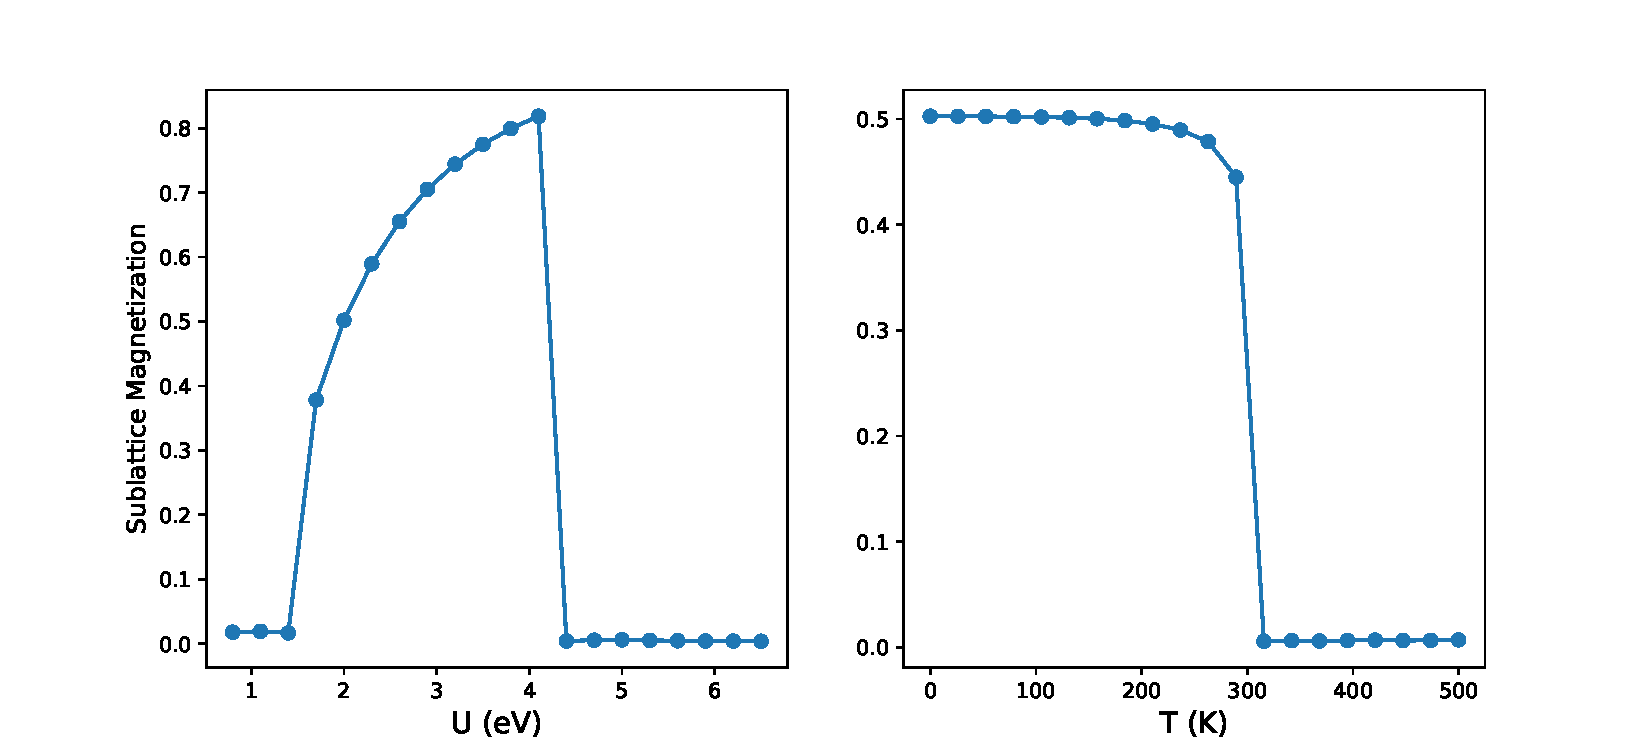
\includegraphics[height=0.5\textwidth, width=1.0\textwidth]
		{pics/magnetization_IPT_AF.pdf}
	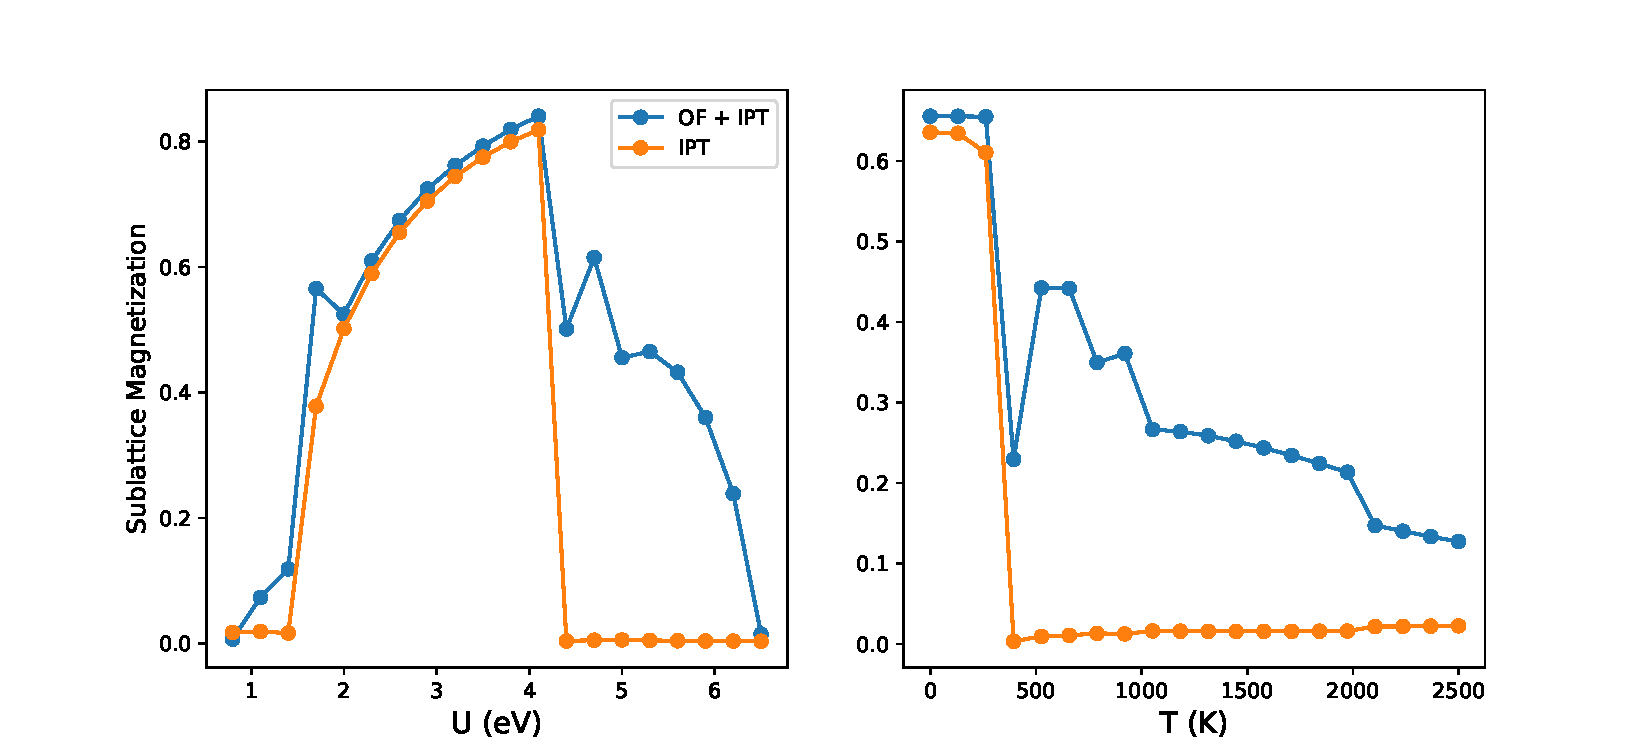
\includegraphics[height=0.5\textwidth, width=1.0\textwidth]
		{pics/magnetization_OFIPT_AF.pdf}
		\caption{(Atas) Evolusi magnetisme dari subkisi terhadap $U$ dan $T$ yang dilakukan dengan metode medan rata-rata. (Tengah) Evolusi magnetisme dari subkisi terhadap $U$ dan $T$ yang dilakukan dengan IPT. (Bawah) Evolusi magnetisme dari subkisi terhadap $U$ dan $T$ yang dilakukan dengan metode IPT+OF.}
\end{figure}
\begin{figure}
	\centering
	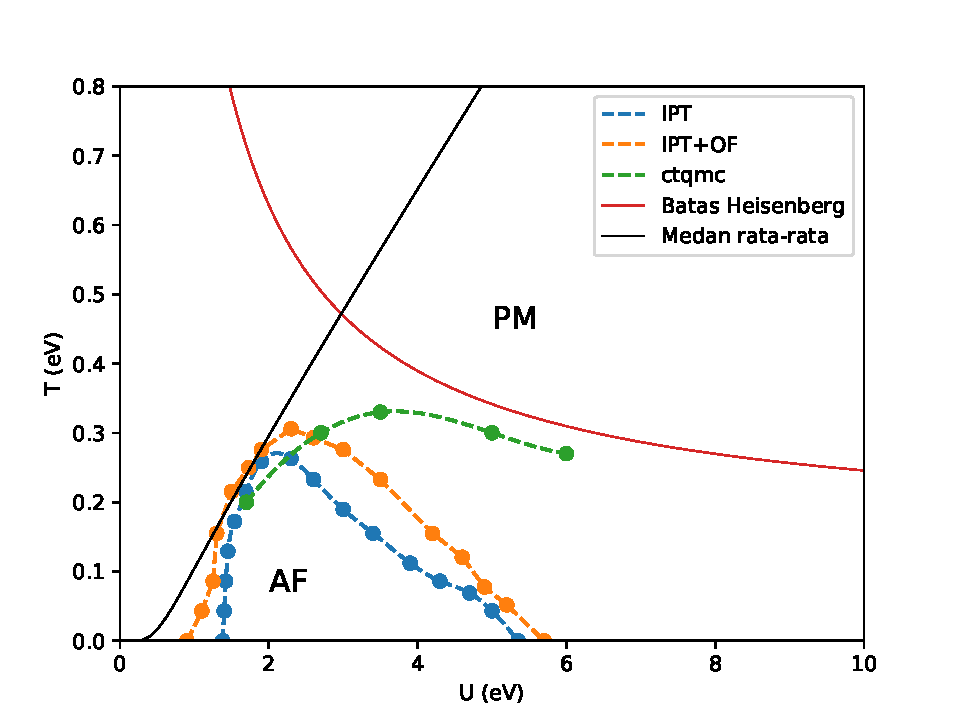
\includegraphics[width=1.0\textwidth]
		{pics/phasediagram_AF.pdf}
		\caption{Diagram Fasa Magnetisme untuk kisi 3D Kubik pada model Hubbard. Kalkulasi dari skripsi ini dilakukan untuk IPT dan IPT+OF. Data CTQMC diambil dari ref\cite{staudt}.}
\end{figure}
%-----------------------------------------------------------------------------%
\chapter{\babLima}
%-----------------------------------------------------------------------------%
\todo{Tambahkan kata-kata pengantar bab 5 disini.}


%-----------------------------------------------------------------------------%
\section{Mengubah Tampilan Teks}
%-----------------------------------------------------------------------------%
Beberapa perintah yang dapat digunakan untuk mengubah tampilan adalah: 
\begin{itemize}
	\item \bslash f \\
		Merupakan alias untuk perintah \bslash textit, contoh 
		\f{contoh hasil tulisan}.
	\item \bslash bi \\
		\bi{Contoh hasil tulisan}.
	\item \bslash bo \\
		\bo{Contoh hasil tulisan}.
	\item \bslash m \\
		\m{Contoh hasil tulisan}.
	\item \bslash mc \\
		\mc{Contoh hasil tulisan}.
	\item \bslash code \\ 
		\code{Contoh hasil tulisan}.
\end{itemize}


%-----------------------------------------------------------------------------%
\section{Memberikan Catatan}
%-----------------------------------------------------------------------------%
Ada dua perintah untuk memberikan catatan penulisan dalam dokumen yang Anda 
kerjakan, yaitu: 
\begin{itemize}
	\item \bslash todo \\
		Contoh: \\ \todo{Contoh bentuk todo.}
	\item \bslash todoCite \\ 
		Contoh: \todoCite
\end{itemize}


%-----------------------------------------------------------------------------%
\section{Menambah Isi Daftar Isi}
%-----------------------------------------------------------------------------%
Terkadang ada kebutuhan untuk memasukan kata-kata tertentu kedalam Daftar Isi. 
Perintah \bslash addChapter dapat digunakan untuk judul bab dalam Daftar isi. 
Contohnya dapat dilihat pada berkas thesis.tex.


%-----------------------------------------------------------------------------%
\section{Memasukan PDF}
%-----------------------------------------------------------------------------%
Untuk memasukan PDF dapat menggunakan perintah \bslash inpdf yang menerima satu 
buah argumen. Argumen ini berisi nama berkas yang akan digabungkan dalam 
laporan. PDF yang dimasukan degnan cara ini akan memiliki header dan footer 
seperti pada halaman lainnya. 

\inpdf{include}

Cara lain untuk memasukan PDF adalah dengan menggunakan perintah \bslash putpdf 
dengan satu argumen yang berisi nama berkas pdf. Berbeda dengan perintah 
sebelumnya, PDF yang dimasukan dengan cara ini tidak akan memiliki footer atau 
header seperti pada halaman lainnya. 

\putpdf{include}


%-----------------------------------------------------------------------------%
\section{Membuat Perintah Baru}
%-----------------------------------------------------------------------------%
Ada dua perintah yang dapat digunakan untuk membuat perintah baru, yaitu: 
\begin{itemize}
	\item \bslash Var \\
		Digunakan untuk membuat perintah baru, namun setiap kata yang diberikan
		akan diproses dahulu menjadi huruf kapital. 
		Contoh jika perintahnya adalah \bslash Var\{adalah\} makan ketika 
		perintah \bslash Var dipanggil, yang akan muncul adalah ADALAH. 
	\item \bslash var \\
		Digunakan untuk membuat perintah atau baru. 
\end{itemize}



%
% Daftar Pustaka
%
% Daftar Pustaka 
% 

% 
% Tambahkan pustaka yang digunakan setelah perintah berikut. 
% 
\begin{thebibliography}{4}

\bibitem{drude}
{Drude, P. \f{Zur Elektronentheorie der Metalle.} Ann. der Phys 306 (3) 566, 1900}

\bibitem{ashcroft-mermin}
{Ashcroft, N. W., and N. D. Mermin. \f{Solid  State  Physics.} Harcourt,Orlando, 1976}

\bibitem{kohn-sham}
{Kohn, W., and L. J. Sham. \f{Self-Consistent Equations Including Exchange and Correlation Effects.} Phys. Rev. A 140 1133, 1965}

\bibitem{boer}
{de Boer, J. H., and E. J. W. Verwey. \f{Semi-conductors with partially and with completely filled 3d-lattice bands.} Proc. Phys. Soc 49 5, 1937}

\bibitem{mott}
{Mott, N. F., and R. Peierls. \f{Discussion of the paper by de Boer and Verwey.} Proc. Phys. Soc 49 72, 1937}

\bibitem{mott-hubbard}
{Rozenberg, M. J, G. Kotliar, and X. Y. Zhang. \f{Mott-Hubbard transition in infinitedimensions. II.} Phys. Rev. B 49: 10181–10193 , 1994}

\bibitem{antiferomagnetik1}
{Hirsch, J. E., and S. Tang. \f{Antiferromagnetism in the Two-Dimensional Hubbard Model.} Phys. Rev. Lett 62: 591–594, 1989}

\bibitem{d-wave}
{Yanagisawa, T. f\f{hysics of the Hubbard model and high temperature supercon-ductivity.} JPCS 108: 012010, 2008}

\bibitem{DMFT}
{Georges, A., et al., ed. \f{Dynamical mean-fieldtheory of strongly correlated fermion systems and the limit of infinite dimensions.} Rev. Mod. Phys 68: 13–125, 1996}

\bibitem{fetter}
{Fetter, A.L., and J.D. Walecka. \f{Quantum Theory of Many-Particle Systems.} Dover Publications, Inc, 2003}

\bibitem{spektral}
{Titchmarsh, C. \f{The theory of functions.}, 1939}

\bibitem{sokhotsi}
{Henrici, Peter. \f{Applied and Computational Complex Analysis, vol. 3.} Willey, John $\&$ Sons, Inc, 1986}

\bibitem{ladder}
{Mattuck, R. \f{A guide to feynman diagram in the many-body problems.}, 1992}

\bibitem{hubbard}
{Hubbard, J. \f{Electron correlations in narrow energy bands.} Proceedings of the Royal Society of London. Series A. Mathematical and Physical Sciences vol. 276 no. 1365 pp. 238–257, 1963}

\bibitem{mott-transition0}
{Strand, H. \f{Critical properties of the mott-hubbard metal-insulatortransition.}, 2011}

\bibitem{magnetic-excitation}
{Karski, M., and G. U. C. Raas. \f{Single-particle dynamics in the vicinity of the mott-hubbard metal-to-insulator transition.} vol. 77 no.7 p. 075116, 2008}

\bibitem{mott-transition1}
{Joo, J., and V. Oudovenko. \f{Quantum Monte Carlo calculation of the finite tem-perature Mott-Hubbard transition.} Phys. Rev. B,  64: 193102, 2001 }

\bibitem{mott-transition2}
{Bulla, R., T. A. Costi, and D. Vollhardt. \f{Finite-temperature numerical renormal-ization group study of the Mott transition.} Phys. Rev. B 64: 045103, 2001}

\bibitem{mott-transition3}
{Capone, M., L. de’ Medici, and A. Georges.  \f{Solving the dynamical mean-fieldtheory at very low temperatures using the Lanczos exact diagonalization.} Phys.Rev. B, 76: 245116, 2007}

\bibitem{mott-transition4}
{Strand, H., et al., ed.  \f{Dynamical mean field theory phase-space extension and critical properties of the finite temperature Mott transition.} Phys. Rev. B 83: 205136, 2011}

\bibitem{staudt}
{Staudt, R., M. Dzierzawa, and A. Muramatsu. \f{Phase diagram of the three-dimensional Hubbard model at half-filling.} Eur. Phys.J. B17 411, 2000}

\bibitem{qmc_tn}
{Hirsch, J. E. \f{Simulations of the three-dimensional Hubbard model: Half-filled band sector.} Phys. Rev. B35, 1851}

\bibitem{dmft_tn}
{Jarrell, M. \f{Hubbard model in infinite dimensions: A quantum Monte Carlo study.} Phys. Rev. Lett 69 168, 1992. }

\bibitem{hartree_tn}
{van Dongen, P. G. J. \f{Extended Hubbard model at weak coupling.} Phys.Rev B50 14016, 1994}

\bibitem{heisenberg_tn}
{Rushbrooke, G. S., G. A. Baker, and P. J. Wood. \f{In Phase Transitions and Critical Phenomena Vol. 3.} Academic Press, New York, 1974}

\bibitem{qmc_tn2}
{Scalettar, R. T., et al., ed. \f{Phase diagram of the half-filled 3D Hubbard model.} Phys. Rev. B39 4711, 1989}

\bibitem{dmft_tn2}
{Ulmke, M., V. Janis, and D. Vollhardt. \f{Anderson-Hubbard model in infinite dimensions} Phys. Rev B51 10411, 1995}

\bibitem{metzner}
{Metzner, W. and D. Vollhardt. \f{Correlated Lattice Fermions in $d = \infty$ Dimensions.} Phys. Rev. Lett, 62: 324–327, 1989}

\bibitem{george}
{Georges, A., and G. Kotliar. \f{Hubbard model in infinite dimensions.} Phys. Rev. B, 45: 6479–6483, 1992}

\bibitem{hfqmc}
{Hirsch, J. E., and R. M. Fye. \f{Monte Carlo Method for Magnetic Impurities in Metals.} Phys. Rev. Lett. 56: 2521–2524, 1986}

\bibitem{ctqmc}
{Werner, P., et al., ed. \f{Continuous-Time Solver for Quantum Impurity Models.} Phys. Rev. Lett. 97: 076405, 2006 }

\bibitem{nrg}
{Wilson, K. G. \f{The renormalization group: Critical phenomena and the Kondo problem.} Rev. Mod. Phys. 47: 773–840, 1975}

\bibitem{dmrg}
{R. White, Steven. \f{Density matrix formulation for quantum renormalization groups.} Phys. Rev. Lett. 69: 2863–2866, 1992}

\bibitem{ipt}
{Kajueter, H., and G. Kotliar. \f{New Iterative Perturbation Scheme for Lattice Modelswith Arbitrary Filling.} Phys. Rev. Lett. 77: 131–134, 1996}

\bibitem{nca}
{Keiter, H, and J. C. Kimball. \f{Perturbation Technique for the Anderson Hamilto-nian.} Phys. Rev. Lett. 25: 672–675, 1970}

\bibitem{sublattice}
{Chitra, R., and G. Kotliar. \f{Dynamical Mean Field Theory of the Antiferromagnetic Metalto Antiferromagnetic Insulator Transition.} Phys. Rev. Lett. 83 2386, 1999}

\bibitem{kent}
{Kent, P. R. C., et al,. ed. \f{Efficient calculation of the antiferromagnetic phase diagram of the 3D Hubbard model} arXiv: cond-mat/0506337, 2005}

\bibitem{rohringer}
{Rohringer, G., et al,. ed. \f{Critical properties of the half-filled Hubbard model in three dimensions} Phys.Rev.Lett. 107 256402, 2011}

\bibitem{daniel}
{Hirschmeier, D., et al,. ed. \f{Mechanisms of finite-temperature magnetism in the three-dimensional Hubbard model} Phys. Rev. B 92 144409, 2015}

\bibitem{dca}
{Hettler, M.H., et al,. ed. \f{Dynamical cluster approximation: Nonlocal dynamics of correlated electron systems} Phys. Rev. B 61 19, 2000}

\bibitem{anna}
{Golubeva, A., A. Sotnikov, and W. Hofstetter. \f{Effects of anisotropy in simple lattice geometries on many-body properties of ultracold fermions in optical lattices} Phys. Rev. A 92 043623, 2015} 

\bibitem{mf}
{Claveau, Y., B. Arnaud, and S.D. Matteo. \f{Mean-field solution of the Hubbard model: the magnetic phase diagram} arXiv:1403.2259, 2014}

\bibitem{el-ph}
{Millis, J., Boris I. Shraiman, and R. Muelle. \f{Dynamic Jahn-Teller effect and colossal magnetoresistance in La$_{1-x}$Sr$_x$MnO$_3$.} Phys. Rev. Lett. 77 1, 1996}

\bibitem{hund}
{Furukawa, N. \f{Thermodynamics of Double Exchange.} J.Phys.Soc. 63 3214, 1994}

\end{thebibliography}



%
% Lampiran 
%
\begin{appendix}
	%
% @author  Andreas Febrian
% @version 1.00 
% 
% Hanya sebuah pembatas bertuliskan LAMPIRAN ditengah halaman. 
% 

\begin{titlepage}
	\centering 
	\vspace*{6cm}
	\noindent \Huge{LAMPIRAN}
	\addChapter{LAMPIRAN}
\end{titlepage}
	\setcounter{page}{2}
	%-----------------------------------------------------------------------------%
\addChapter{Lampiran 1}
\chapter*{Lampiran 1}
%-----------------------------------------------------------------------------%
\end{appendix}

\end{document}